% Created by tikzDevice version 0.12.3.1 on 2021-12-03 16:21:44
% !TEX encoding = UTF-8 Unicode
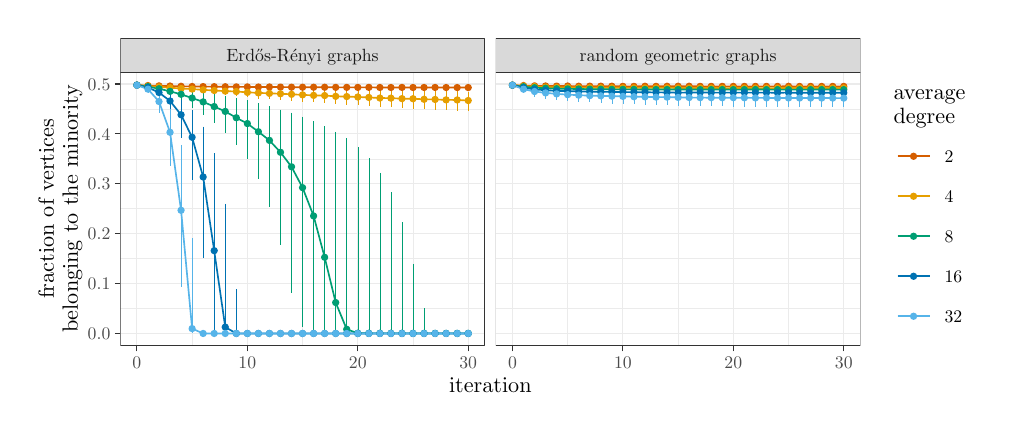
\begin{tikzpicture}[x=1pt,y=1pt]
\definecolor{fillColor}{RGB}{255,255,255}
\path[use as bounding box,fill=fillColor,fill opacity=0.00] (0,0) rectangle (346.90,137.31);
\begin{scope}
\path[clip] (  0.00,  0.00) rectangle (346.90,137.31);
\definecolor{drawColor}{RGB}{255,255,255}
\definecolor{fillColor}{RGB}{255,255,255}

\path[draw=drawColor,line width= 0.4pt,line join=round,line cap=round,fill=fillColor] (  0.00,  0.00) rectangle (346.90,137.31);
\end{scope}
\begin{scope}
\path[clip] ( 33.48, 22.32) rectangle (165.18,121.26);
\definecolor{fillColor}{RGB}{255,255,255}

\path[fill=fillColor] ( 33.48, 22.32) rectangle (165.18,121.26);
\definecolor{drawColor}{gray}{0.92}

\path[draw=drawColor,line width= 0.2pt,line join=round] ( 33.48, 35.83) --
	(165.18, 35.83);

\path[draw=drawColor,line width= 0.2pt,line join=round] ( 33.48, 53.85) --
	(165.18, 53.85);

\path[draw=drawColor,line width= 0.2pt,line join=round] ( 33.48, 71.88) --
	(165.18, 71.88);

\path[draw=drawColor,line width= 0.2pt,line join=round] ( 33.48, 89.90) --
	(165.18, 89.90);

\path[draw=drawColor,line width= 0.2pt,line join=round] ( 33.48,107.92) --
	(165.18,107.92);

\path[draw=drawColor,line width= 0.2pt,line join=round] ( 59.42, 22.32) --
	( 59.42,121.26);

\path[draw=drawColor,line width= 0.2pt,line join=round] ( 99.33, 22.32) --
	( 99.33,121.26);

\path[draw=drawColor,line width= 0.2pt,line join=round] (139.24, 22.32) --
	(139.24,121.26);

\path[draw=drawColor,line width= 0.4pt,line join=round] ( 33.48, 26.81) --
	(165.18, 26.81);

\path[draw=drawColor,line width= 0.4pt,line join=round] ( 33.48, 44.84) --
	(165.18, 44.84);

\path[draw=drawColor,line width= 0.4pt,line join=round] ( 33.48, 62.86) --
	(165.18, 62.86);

\path[draw=drawColor,line width= 0.4pt,line join=round] ( 33.48, 80.89) --
	(165.18, 80.89);

\path[draw=drawColor,line width= 0.4pt,line join=round] ( 33.48, 98.91) --
	(165.18, 98.91);

\path[draw=drawColor,line width= 0.4pt,line join=round] ( 33.48,116.94) --
	(165.18,116.94);

\path[draw=drawColor,line width= 0.4pt,line join=round] ( 39.47, 22.32) --
	( 39.47,121.26);

\path[draw=drawColor,line width= 0.4pt,line join=round] ( 79.38, 22.32) --
	( 79.38,121.26);

\path[draw=drawColor,line width= 0.4pt,line join=round] (119.29, 22.32) --
	(119.29,121.26);

\path[draw=drawColor,line width= 0.4pt,line join=round] (159.19, 22.32) --
	(159.19,121.26);
\definecolor{drawColor}{RGB}{213,94,0}

\path[draw=drawColor,line width= 0.2pt,line join=round] ( 39.47,116.76) --
	( 39.47,116.76);

\path[draw=drawColor,line width= 0.2pt,line join=round] ( 39.47,116.76) --
	( 39.47,116.27);

\path[draw=drawColor,line width= 0.2pt,line join=round] ( 39.47,116.27) --
	( 39.47,116.27);

\path[draw=drawColor,line width= 0.2pt,line join=round] ( 43.46,116.68) --
	( 43.46,116.68);

\path[draw=drawColor,line width= 0.2pt,line join=round] ( 43.46,116.68) --
	( 43.46,116.00);

\path[draw=drawColor,line width= 0.2pt,line join=round] ( 43.46,116.00) --
	( 43.46,116.00);

\path[draw=drawColor,line width= 0.2pt,line join=round] ( 47.45,116.62) --
	( 47.45,116.62);

\path[draw=drawColor,line width= 0.2pt,line join=round] ( 47.45,116.62) --
	( 47.45,115.82);

\path[draw=drawColor,line width= 0.2pt,line join=round] ( 47.45,115.82) --
	( 47.45,115.82);

\path[draw=drawColor,line width= 0.2pt,line join=round] ( 51.44,116.57) --
	( 51.44,116.57);

\path[draw=drawColor,line width= 0.2pt,line join=round] ( 51.44,116.57) --
	( 51.44,115.68);

\path[draw=drawColor,line width= 0.2pt,line join=round] ( 51.44,115.68) --
	( 51.44,115.68);

\path[draw=drawColor,line width= 0.2pt,line join=round] ( 55.43,116.55) --
	( 55.43,116.55);

\path[draw=drawColor,line width= 0.2pt,line join=round] ( 55.43,116.55) --
	( 55.43,115.57);

\path[draw=drawColor,line width= 0.2pt,line join=round] ( 55.43,115.57) --
	( 55.43,115.57);

\path[draw=drawColor,line width= 0.2pt,line join=round] ( 59.42,116.53) --
	( 59.42,116.53);

\path[draw=drawColor,line width= 0.2pt,line join=round] ( 59.42,116.53) --
	( 59.42,115.54);

\path[draw=drawColor,line width= 0.2pt,line join=round] ( 59.42,115.54) --
	( 59.42,115.54);

\path[draw=drawColor,line width= 0.2pt,line join=round] ( 63.41,116.52) --
	( 63.41,116.52);

\path[draw=drawColor,line width= 0.2pt,line join=round] ( 63.41,116.52) --
	( 63.41,115.40);

\path[draw=drawColor,line width= 0.2pt,line join=round] ( 63.41,115.40) --
	( 63.41,115.40);

\path[draw=drawColor,line width= 0.2pt,line join=round] ( 67.40,116.50) --
	( 67.40,116.50);

\path[draw=drawColor,line width= 0.2pt,line join=round] ( 67.40,116.50) --
	( 67.40,115.38);

\path[draw=drawColor,line width= 0.2pt,line join=round] ( 67.40,115.38) --
	( 67.40,115.38);

\path[draw=drawColor,line width= 0.2pt,line join=round] ( 71.39,116.48) --
	( 71.39,116.48);

\path[draw=drawColor,line width= 0.2pt,line join=round] ( 71.39,116.48) --
	( 71.39,115.30);

\path[draw=drawColor,line width= 0.2pt,line join=round] ( 71.39,115.30) --
	( 71.39,115.30);

\path[draw=drawColor,line width= 0.2pt,line join=round] ( 75.39,116.42) --
	( 75.39,116.42);

\path[draw=drawColor,line width= 0.2pt,line join=round] ( 75.39,116.42) --
	( 75.39,115.25);

\path[draw=drawColor,line width= 0.2pt,line join=round] ( 75.39,115.25) --
	( 75.39,115.25);

\path[draw=drawColor,line width= 0.2pt,line join=round] ( 79.38,116.42) --
	( 79.38,116.42);

\path[draw=drawColor,line width= 0.2pt,line join=round] ( 79.38,116.42) --
	( 79.38,115.22);

\path[draw=drawColor,line width= 0.2pt,line join=round] ( 79.38,115.22) --
	( 79.38,115.22);

\path[draw=drawColor,line width= 0.2pt,line join=round] ( 83.37,116.40) --
	( 83.37,116.40);

\path[draw=drawColor,line width= 0.2pt,line join=round] ( 83.37,116.40) --
	( 83.37,115.18);

\path[draw=drawColor,line width= 0.2pt,line join=round] ( 83.37,115.18) --
	( 83.37,115.18);

\path[draw=drawColor,line width= 0.2pt,line join=round] ( 87.36,116.41) --
	( 87.36,116.41);

\path[draw=drawColor,line width= 0.2pt,line join=round] ( 87.36,116.41) --
	( 87.36,115.18);

\path[draw=drawColor,line width= 0.2pt,line join=round] ( 87.36,115.18) --
	( 87.36,115.18);

\path[draw=drawColor,line width= 0.2pt,line join=round] ( 91.35,116.39) --
	( 91.35,116.39);

\path[draw=drawColor,line width= 0.2pt,line join=round] ( 91.35,116.39) --
	( 91.35,115.12);

\path[draw=drawColor,line width= 0.2pt,line join=round] ( 91.35,115.12) --
	( 91.35,115.12);

\path[draw=drawColor,line width= 0.2pt,line join=round] ( 95.34,116.40) --
	( 95.34,116.40);

\path[draw=drawColor,line width= 0.2pt,line join=round] ( 95.34,116.40) --
	( 95.34,115.10);

\path[draw=drawColor,line width= 0.2pt,line join=round] ( 95.34,115.10) --
	( 95.34,115.10);

\path[draw=drawColor,line width= 0.2pt,line join=round] ( 99.33,116.35) --
	( 99.33,116.35);

\path[draw=drawColor,line width= 0.2pt,line join=round] ( 99.33,116.35) --
	( 99.33,115.01);

\path[draw=drawColor,line width= 0.2pt,line join=round] ( 99.33,115.01) --
	( 99.33,115.01);

\path[draw=drawColor,line width= 0.2pt,line join=round] (103.32,116.35) --
	(103.32,116.35);

\path[draw=drawColor,line width= 0.2pt,line join=round] (103.32,116.35) --
	(103.32,114.99);

\path[draw=drawColor,line width= 0.2pt,line join=round] (103.32,114.99) --
	(103.32,114.99);

\path[draw=drawColor,line width= 0.2pt,line join=round] (107.31,116.37) --
	(107.31,116.37);

\path[draw=drawColor,line width= 0.2pt,line join=round] (107.31,116.37) --
	(107.31,115.02);

\path[draw=drawColor,line width= 0.2pt,line join=round] (107.31,115.02) --
	(107.31,115.02);

\path[draw=drawColor,line width= 0.2pt,line join=round] (111.30,116.40) --
	(111.30,116.40);

\path[draw=drawColor,line width= 0.2pt,line join=round] (111.30,116.40) --
	(111.30,115.02);

\path[draw=drawColor,line width= 0.2pt,line join=round] (111.30,115.02) --
	(111.30,115.02);

\path[draw=drawColor,line width= 0.2pt,line join=round] (115.29,116.37) --
	(115.29,116.37);

\path[draw=drawColor,line width= 0.2pt,line join=round] (115.29,116.37) --
	(115.29,114.97);

\path[draw=drawColor,line width= 0.2pt,line join=round] (115.29,114.97) --
	(115.29,114.97);

\path[draw=drawColor,line width= 0.2pt,line join=round] (119.29,116.36) --
	(119.29,116.36);

\path[draw=drawColor,line width= 0.2pt,line join=round] (119.29,116.36) --
	(119.29,114.93);

\path[draw=drawColor,line width= 0.2pt,line join=round] (119.29,114.93) --
	(119.29,114.93);

\path[draw=drawColor,line width= 0.2pt,line join=round] (123.28,116.35) --
	(123.28,116.35);

\path[draw=drawColor,line width= 0.2pt,line join=round] (123.28,116.35) --
	(123.28,114.96);

\path[draw=drawColor,line width= 0.2pt,line join=round] (123.28,114.96) --
	(123.28,114.96);

\path[draw=drawColor,line width= 0.2pt,line join=round] (127.27,116.32) --
	(127.27,116.32);

\path[draw=drawColor,line width= 0.2pt,line join=round] (127.27,116.32) --
	(127.27,114.88);

\path[draw=drawColor,line width= 0.2pt,line join=round] (127.27,114.88) --
	(127.27,114.88);

\path[draw=drawColor,line width= 0.2pt,line join=round] (131.26,116.35) --
	(131.26,116.35);

\path[draw=drawColor,line width= 0.2pt,line join=round] (131.26,116.35) --
	(131.26,114.87);

\path[draw=drawColor,line width= 0.2pt,line join=round] (131.26,114.87) --
	(131.26,114.87);

\path[draw=drawColor,line width= 0.2pt,line join=round] (135.25,116.38) --
	(135.25,116.38);

\path[draw=drawColor,line width= 0.2pt,line join=round] (135.25,116.38) --
	(135.25,114.77);

\path[draw=drawColor,line width= 0.2pt,line join=round] (135.25,114.77) --
	(135.25,114.77);

\path[draw=drawColor,line width= 0.2pt,line join=round] (139.24,116.37) --
	(139.24,116.37);

\path[draw=drawColor,line width= 0.2pt,line join=round] (139.24,116.37) --
	(139.24,114.82);

\path[draw=drawColor,line width= 0.2pt,line join=round] (139.24,114.82) --
	(139.24,114.82);

\path[draw=drawColor,line width= 0.2pt,line join=round] (143.23,116.32) --
	(143.23,116.32);

\path[draw=drawColor,line width= 0.2pt,line join=round] (143.23,116.32) --
	(143.23,114.77);

\path[draw=drawColor,line width= 0.2pt,line join=round] (143.23,114.77) --
	(143.23,114.77);

\path[draw=drawColor,line width= 0.2pt,line join=round] (147.22,116.31) --
	(147.22,116.31);

\path[draw=drawColor,line width= 0.2pt,line join=round] (147.22,116.31) --
	(147.22,114.81);

\path[draw=drawColor,line width= 0.2pt,line join=round] (147.22,114.81) --
	(147.22,114.81);

\path[draw=drawColor,line width= 0.2pt,line join=round] (151.21,116.31) --
	(151.21,116.31);

\path[draw=drawColor,line width= 0.2pt,line join=round] (151.21,116.31) --
	(151.21,114.75);

\path[draw=drawColor,line width= 0.2pt,line join=round] (151.21,114.75) --
	(151.21,114.75);

\path[draw=drawColor,line width= 0.2pt,line join=round] (155.20,116.31) --
	(155.20,116.31);

\path[draw=drawColor,line width= 0.2pt,line join=round] (155.20,116.31) --
	(155.20,114.82);

\path[draw=drawColor,line width= 0.2pt,line join=round] (155.20,114.82) --
	(155.20,114.82);

\path[draw=drawColor,line width= 0.2pt,line join=round] (159.19,116.33) --
	(159.19,116.33);

\path[draw=drawColor,line width= 0.2pt,line join=round] (159.19,116.33) --
	(159.19,114.76);

\path[draw=drawColor,line width= 0.2pt,line join=round] (159.19,114.76) --
	(159.19,114.76);
\definecolor{drawColor}{RGB}{230,159,0}

\path[draw=drawColor,line width= 0.2pt,line join=round] ( 39.47,116.75) --
	( 39.47,116.75);

\path[draw=drawColor,line width= 0.2pt,line join=round] ( 39.47,116.75) --
	( 39.47,116.25);

\path[draw=drawColor,line width= 0.2pt,line join=round] ( 39.47,116.25) --
	( 39.47,116.25);

\path[draw=drawColor,line width= 0.2pt,line join=round] ( 43.46,116.61) --
	( 43.46,116.61);

\path[draw=drawColor,line width= 0.2pt,line join=round] ( 43.46,116.61) --
	( 43.46,115.71);

\path[draw=drawColor,line width= 0.2pt,line join=round] ( 43.46,115.71) --
	( 43.46,115.71);

\path[draw=drawColor,line width= 0.2pt,line join=round] ( 47.45,116.46) --
	( 47.45,116.46);

\path[draw=drawColor,line width= 0.2pt,line join=round] ( 47.45,116.46) --
	( 47.45,115.22);

\path[draw=drawColor,line width= 0.2pt,line join=round] ( 47.45,115.22) --
	( 47.45,115.22);

\path[draw=drawColor,line width= 0.2pt,line join=round] ( 51.44,116.32) --
	( 51.44,116.32);

\path[draw=drawColor,line width= 0.2pt,line join=round] ( 51.44,116.32) --
	( 51.44,114.78);

\path[draw=drawColor,line width= 0.2pt,line join=round] ( 51.44,114.78) --
	( 51.44,114.78);

\path[draw=drawColor,line width= 0.2pt,line join=round] ( 55.43,116.21) --
	( 55.43,116.21);

\path[draw=drawColor,line width= 0.2pt,line join=round] ( 55.43,116.21) --
	( 55.43,114.36);

\path[draw=drawColor,line width= 0.2pt,line join=round] ( 55.43,114.36) --
	( 55.43,114.36);

\path[draw=drawColor,line width= 0.2pt,line join=round] ( 59.42,116.08) --
	( 59.42,116.08);

\path[draw=drawColor,line width= 0.2pt,line join=round] ( 59.42,116.08) --
	( 59.42,113.92);

\path[draw=drawColor,line width= 0.2pt,line join=round] ( 59.42,113.92) --
	( 59.42,113.92);

\path[draw=drawColor,line width= 0.2pt,line join=round] ( 63.41,115.98) --
	( 63.41,115.98);

\path[draw=drawColor,line width= 0.2pt,line join=round] ( 63.41,115.98) --
	( 63.41,113.58);

\path[draw=drawColor,line width= 0.2pt,line join=round] ( 63.41,113.58) --
	( 63.41,113.58);

\path[draw=drawColor,line width= 0.2pt,line join=round] ( 67.40,115.88) --
	( 67.40,115.88);

\path[draw=drawColor,line width= 0.2pt,line join=round] ( 67.40,115.88) --
	( 67.40,113.19);

\path[draw=drawColor,line width= 0.2pt,line join=round] ( 67.40,113.19) --
	( 67.40,113.19);

\path[draw=drawColor,line width= 0.2pt,line join=round] ( 71.39,115.79) --
	( 71.39,115.79);

\path[draw=drawColor,line width= 0.2pt,line join=round] ( 71.39,115.79) --
	( 71.39,112.80);

\path[draw=drawColor,line width= 0.2pt,line join=round] ( 71.39,112.80) --
	( 71.39,112.80);

\path[draw=drawColor,line width= 0.2pt,line join=round] ( 75.39,115.67) --
	( 75.39,115.67);

\path[draw=drawColor,line width= 0.2pt,line join=round] ( 75.39,115.67) --
	( 75.39,112.44);

\path[draw=drawColor,line width= 0.2pt,line join=round] ( 75.39,112.44) --
	( 75.39,112.44);

\path[draw=drawColor,line width= 0.2pt,line join=round] ( 79.38,115.56) --
	( 79.38,115.56);

\path[draw=drawColor,line width= 0.2pt,line join=round] ( 79.38,115.56) --
	( 79.38,112.15);

\path[draw=drawColor,line width= 0.2pt,line join=round] ( 79.38,112.15) --
	( 79.38,112.15);

\path[draw=drawColor,line width= 0.2pt,line join=round] ( 83.37,115.46) --
	( 83.37,115.46);

\path[draw=drawColor,line width= 0.2pt,line join=round] ( 83.37,115.46) --
	( 83.37,111.70);

\path[draw=drawColor,line width= 0.2pt,line join=round] ( 83.37,111.70) --
	( 83.37,111.70);

\path[draw=drawColor,line width= 0.2pt,line join=round] ( 87.36,115.39) --
	( 87.36,115.39);

\path[draw=drawColor,line width= 0.2pt,line join=round] ( 87.36,115.39) --
	( 87.36,111.50);

\path[draw=drawColor,line width= 0.2pt,line join=round] ( 87.36,111.50) --
	( 87.36,111.50);

\path[draw=drawColor,line width= 0.2pt,line join=round] ( 91.35,115.30) --
	( 91.35,115.30);

\path[draw=drawColor,line width= 0.2pt,line join=round] ( 91.35,115.30) --
	( 91.35,111.12);

\path[draw=drawColor,line width= 0.2pt,line join=round] ( 91.35,111.12) --
	( 91.35,111.12);

\path[draw=drawColor,line width= 0.2pt,line join=round] ( 95.34,115.29) --
	( 95.34,115.29);

\path[draw=drawColor,line width= 0.2pt,line join=round] ( 95.34,115.29) --
	( 95.34,110.82);

\path[draw=drawColor,line width= 0.2pt,line join=round] ( 95.34,110.82) --
	( 95.34,110.82);

\path[draw=drawColor,line width= 0.2pt,line join=round] ( 99.33,115.15) --
	( 99.33,115.15);

\path[draw=drawColor,line width= 0.2pt,line join=round] ( 99.33,115.15) --
	( 99.33,110.58);

\path[draw=drawColor,line width= 0.2pt,line join=round] ( 99.33,110.58) --
	( 99.33,110.58);

\path[draw=drawColor,line width= 0.2pt,line join=round] (103.32,115.08) --
	(103.32,115.08);

\path[draw=drawColor,line width= 0.2pt,line join=round] (103.32,115.08) --
	(103.32,110.34);

\path[draw=drawColor,line width= 0.2pt,line join=round] (103.32,110.34) --
	(103.32,110.34);

\path[draw=drawColor,line width= 0.2pt,line join=round] (107.31,114.96) --
	(107.31,114.96);

\path[draw=drawColor,line width= 0.2pt,line join=round] (107.31,114.96) --
	(107.31,110.02);

\path[draw=drawColor,line width= 0.2pt,line join=round] (107.31,110.02) --
	(107.31,110.02);

\path[draw=drawColor,line width= 0.2pt,line join=round] (111.30,114.94) --
	(111.30,114.94);

\path[draw=drawColor,line width= 0.2pt,line join=round] (111.30,114.94) --
	(111.30,109.81);

\path[draw=drawColor,line width= 0.2pt,line join=round] (111.30,109.81) --
	(111.30,109.81);

\path[draw=drawColor,line width= 0.2pt,line join=round] (115.29,114.84) --
	(115.29,114.84);

\path[draw=drawColor,line width= 0.2pt,line join=round] (115.29,114.84) --
	(115.29,109.48);

\path[draw=drawColor,line width= 0.2pt,line join=round] (115.29,109.48) --
	(115.29,109.48);

\path[draw=drawColor,line width= 0.2pt,line join=round] (119.29,114.73) --
	(119.29,114.73);

\path[draw=drawColor,line width= 0.2pt,line join=round] (119.29,114.73) --
	(119.29,109.33);

\path[draw=drawColor,line width= 0.2pt,line join=round] (119.29,109.33) --
	(119.29,109.33);

\path[draw=drawColor,line width= 0.2pt,line join=round] (123.28,114.70) --
	(123.28,114.70);

\path[draw=drawColor,line width= 0.2pt,line join=round] (123.28,114.70) --
	(123.28,109.06);

\path[draw=drawColor,line width= 0.2pt,line join=round] (123.28,109.06) --
	(123.28,109.06);

\path[draw=drawColor,line width= 0.2pt,line join=round] (127.27,114.63) --
	(127.27,114.63);

\path[draw=drawColor,line width= 0.2pt,line join=round] (127.27,114.63) --
	(127.27,108.79);

\path[draw=drawColor,line width= 0.2pt,line join=round] (127.27,108.79) --
	(127.27,108.79);

\path[draw=drawColor,line width= 0.2pt,line join=round] (131.26,114.52) --
	(131.26,114.52);

\path[draw=drawColor,line width= 0.2pt,line join=round] (131.26,114.52) --
	(131.26,108.51);

\path[draw=drawColor,line width= 0.2pt,line join=round] (131.26,108.51) --
	(131.26,108.51);

\path[draw=drawColor,line width= 0.2pt,line join=round] (135.25,114.55) --
	(135.25,114.55);

\path[draw=drawColor,line width= 0.2pt,line join=round] (135.25,114.55) --
	(135.25,108.34);

\path[draw=drawColor,line width= 0.2pt,line join=round] (135.25,108.34) --
	(135.25,108.34);

\path[draw=drawColor,line width= 0.2pt,line join=round] (139.24,114.49) --
	(139.24,114.49);

\path[draw=drawColor,line width= 0.2pt,line join=round] (139.24,114.49) --
	(139.24,108.04);

\path[draw=drawColor,line width= 0.2pt,line join=round] (139.24,108.04) --
	(139.24,108.04);

\path[draw=drawColor,line width= 0.2pt,line join=round] (143.23,114.41) --
	(143.23,114.41);

\path[draw=drawColor,line width= 0.2pt,line join=round] (143.23,114.41) --
	(143.23,107.92);

\path[draw=drawColor,line width= 0.2pt,line join=round] (143.23,107.92) --
	(143.23,107.92);

\path[draw=drawColor,line width= 0.2pt,line join=round] (147.22,114.40) --
	(147.22,114.40);

\path[draw=drawColor,line width= 0.2pt,line join=round] (147.22,114.40) --
	(147.22,107.68);

\path[draw=drawColor,line width= 0.2pt,line join=round] (147.22,107.68) --
	(147.22,107.68);

\path[draw=drawColor,line width= 0.2pt,line join=round] (151.21,114.37) --
	(151.21,114.37);

\path[draw=drawColor,line width= 0.2pt,line join=round] (151.21,114.37) --
	(151.21,107.52);

\path[draw=drawColor,line width= 0.2pt,line join=round] (151.21,107.52) --
	(151.21,107.52);

\path[draw=drawColor,line width= 0.2pt,line join=round] (155.20,114.25) --
	(155.20,114.25);

\path[draw=drawColor,line width= 0.2pt,line join=round] (155.20,114.25) --
	(155.20,107.28);

\path[draw=drawColor,line width= 0.2pt,line join=round] (155.20,107.28) --
	(155.20,107.28);

\path[draw=drawColor,line width= 0.2pt,line join=round] (159.19,114.23) --
	(159.19,114.23);

\path[draw=drawColor,line width= 0.2pt,line join=round] (159.19,114.23) --
	(159.19,107.09);

\path[draw=drawColor,line width= 0.2pt,line join=round] (159.19,107.09) --
	(159.19,107.09);
\definecolor{drawColor}{RGB}{0,158,115}

\path[draw=drawColor,line width= 0.2pt,line join=round] ( 39.47,116.76) --
	( 39.47,116.76);

\path[draw=drawColor,line width= 0.2pt,line join=round] ( 39.47,116.76) --
	( 39.47,116.30);

\path[draw=drawColor,line width= 0.2pt,line join=round] ( 39.47,116.30) --
	( 39.47,116.30);

\path[draw=drawColor,line width= 0.2pt,line join=round] ( 43.46,116.51) --
	( 43.46,116.51);

\path[draw=drawColor,line width= 0.2pt,line join=round] ( 43.46,116.51) --
	( 43.46,115.37);

\path[draw=drawColor,line width= 0.2pt,line join=round] ( 43.46,115.37) --
	( 43.46,115.37);

\path[draw=drawColor,line width= 0.2pt,line join=round] ( 47.45,116.21) --
	( 47.45,116.21);

\path[draw=drawColor,line width= 0.2pt,line join=round] ( 47.45,116.21) --
	( 47.45,114.04);

\path[draw=drawColor,line width= 0.2pt,line join=round] ( 47.45,114.04) --
	( 47.45,114.04);

\path[draw=drawColor,line width= 0.2pt,line join=round] ( 51.44,115.83) --
	( 51.44,115.83);

\path[draw=drawColor,line width= 0.2pt,line join=round] ( 51.44,115.83) --
	( 51.44,112.44);

\path[draw=drawColor,line width= 0.2pt,line join=round] ( 51.44,112.44) --
	( 51.44,112.44);

\path[draw=drawColor,line width= 0.2pt,line join=round] ( 55.43,115.37) --
	( 55.43,115.37);

\path[draw=drawColor,line width= 0.2pt,line join=round] ( 55.43,115.37) --
	( 55.43,110.45);

\path[draw=drawColor,line width= 0.2pt,line join=round] ( 55.43,110.45) --
	( 55.43,110.45);

\path[draw=drawColor,line width= 0.2pt,line join=round] ( 59.42,114.82) --
	( 59.42,114.82);

\path[draw=drawColor,line width= 0.2pt,line join=round] ( 59.42,114.82) --
	( 59.42,108.28);

\path[draw=drawColor,line width= 0.2pt,line join=round] ( 59.42,108.28) --
	( 59.42,108.28);

\path[draw=drawColor,line width= 0.2pt,line join=round] ( 63.41,114.16) --
	( 63.41,114.16);

\path[draw=drawColor,line width= 0.2pt,line join=round] ( 63.41,114.16) --
	( 63.41,105.73);

\path[draw=drawColor,line width= 0.2pt,line join=round] ( 63.41,105.73) --
	( 63.41,105.73);

\path[draw=drawColor,line width= 0.2pt,line join=round] ( 67.40,113.53) --
	( 67.40,113.53);

\path[draw=drawColor,line width= 0.2pt,line join=round] ( 67.40,113.53) --
	( 67.40,102.79);

\path[draw=drawColor,line width= 0.2pt,line join=round] ( 67.40,102.79) --
	( 67.40,102.79);

\path[draw=drawColor,line width= 0.2pt,line join=round] ( 71.39,112.74) --
	( 71.39,112.74);

\path[draw=drawColor,line width= 0.2pt,line join=round] ( 71.39,112.74) --
	( 71.39, 99.26);

\path[draw=drawColor,line width= 0.2pt,line join=round] ( 71.39, 99.26) --
	( 71.39, 99.26);

\path[draw=drawColor,line width= 0.2pt,line join=round] ( 75.39,111.87) --
	( 75.39,111.87);

\path[draw=drawColor,line width= 0.2pt,line join=round] ( 75.39,111.87) --
	( 75.39, 94.98);

\path[draw=drawColor,line width= 0.2pt,line join=round] ( 75.39, 94.98) --
	( 75.39, 94.98);

\path[draw=drawColor,line width= 0.2pt,line join=round] ( 79.38,111.02) --
	( 79.38,111.02);

\path[draw=drawColor,line width= 0.2pt,line join=round] ( 79.38,111.02) --
	( 79.38, 89.71);

\path[draw=drawColor,line width= 0.2pt,line join=round] ( 79.38, 89.71) --
	( 79.38, 89.71);

\path[draw=drawColor,line width= 0.2pt,line join=round] ( 83.37,109.97) --
	( 83.37,109.97);

\path[draw=drawColor,line width= 0.2pt,line join=round] ( 83.37,109.97) --
	( 83.37, 82.52);

\path[draw=drawColor,line width= 0.2pt,line join=round] ( 83.37, 82.52) --
	( 83.37, 82.52);

\path[draw=drawColor,line width= 0.2pt,line join=round] ( 87.36,108.87) --
	( 87.36,108.87);

\path[draw=drawColor,line width= 0.2pt,line join=round] ( 87.36,108.87) --
	( 87.36, 72.61);

\path[draw=drawColor,line width= 0.2pt,line join=round] ( 87.36, 72.61) --
	( 87.36, 72.61);

\path[draw=drawColor,line width= 0.2pt,line join=round] ( 91.35,107.72) --
	( 91.35,107.72);

\path[draw=drawColor,line width= 0.2pt,line join=round] ( 91.35,107.72) --
	( 91.35, 58.61);

\path[draw=drawColor,line width= 0.2pt,line join=round] ( 91.35, 58.61) --
	( 91.35, 58.61);

\path[draw=drawColor,line width= 0.2pt,line join=round] ( 95.34,106.60) --
	( 95.34,106.60);

\path[draw=drawColor,line width= 0.2pt,line join=round] ( 95.34,106.60) --
	( 95.34, 41.48);

\path[draw=drawColor,line width= 0.2pt,line join=round] ( 95.34, 41.48) --
	( 95.34, 41.48);

\path[draw=drawColor,line width= 0.2pt,line join=round] ( 99.33,105.06) --
	( 99.33,105.06);

\path[draw=drawColor,line width= 0.2pt,line join=round] ( 99.33,105.06) --
	( 99.33, 29.31);

\path[draw=drawColor,line width= 0.2pt,line join=round] ( 99.33, 29.31) --
	( 99.33, 29.31);

\path[draw=drawColor,line width= 0.2pt,line join=round] (103.32,103.58) --
	(103.32,103.58);

\path[draw=drawColor,line width= 0.2pt,line join=round] (103.32,103.58) --
	(103.32, 26.96);

\path[draw=drawColor,line width= 0.2pt,line join=round] (103.32, 26.96) --
	(103.32, 26.96);

\path[draw=drawColor,line width= 0.2pt,line join=round] (107.31,101.75) --
	(107.31,101.75);

\path[draw=drawColor,line width= 0.2pt,line join=round] (107.31,101.75) --
	(107.31, 26.86);

\path[draw=drawColor,line width= 0.2pt,line join=round] (107.31, 26.86) --
	(107.31, 26.86);

\path[draw=drawColor,line width= 0.2pt,line join=round] (111.30, 99.70) --
	(111.30, 99.70);

\path[draw=drawColor,line width= 0.2pt,line join=round] (111.30, 99.70) --
	(111.30, 26.85);

\path[draw=drawColor,line width= 0.2pt,line join=round] (111.30, 26.85) --
	(111.30, 26.85);

\path[draw=drawColor,line width= 0.2pt,line join=round] (115.29, 97.33) --
	(115.29, 97.33);

\path[draw=drawColor,line width= 0.2pt,line join=round] (115.29, 97.33) --
	(115.29, 26.85);

\path[draw=drawColor,line width= 0.2pt,line join=round] (115.29, 26.85) --
	(115.29, 26.85);

\path[draw=drawColor,line width= 0.2pt,line join=round] (119.29, 94.01) --
	(119.29, 94.01);

\path[draw=drawColor,line width= 0.2pt,line join=round] (119.29, 94.01) --
	(119.29, 26.84);

\path[draw=drawColor,line width= 0.2pt,line join=round] (119.29, 26.84) --
	(119.29, 26.84);

\path[draw=drawColor,line width= 0.2pt,line join=round] (123.28, 90.20) --
	(123.28, 90.20);

\path[draw=drawColor,line width= 0.2pt,line join=round] (123.28, 90.20) --
	(123.28, 26.84);

\path[draw=drawColor,line width= 0.2pt,line join=round] (123.28, 26.84) --
	(123.28, 26.84);

\path[draw=drawColor,line width= 0.2pt,line join=round] (127.27, 84.88) --
	(127.27, 84.88);

\path[draw=drawColor,line width= 0.2pt,line join=round] (127.27, 84.88) --
	(127.27, 26.84);

\path[draw=drawColor,line width= 0.2pt,line join=round] (127.27, 26.84) --
	(127.27, 26.84);

\path[draw=drawColor,line width= 0.2pt,line join=round] (131.26, 77.76) --
	(131.26, 77.76);

\path[draw=drawColor,line width= 0.2pt,line join=round] (131.26, 77.76) --
	(131.26, 26.84);

\path[draw=drawColor,line width= 0.2pt,line join=round] (131.26, 26.84) --
	(131.26, 26.84);

\path[draw=drawColor,line width= 0.2pt,line join=round] (135.25, 67.01) --
	(135.25, 67.01);

\path[draw=drawColor,line width= 0.2pt,line join=round] (135.25, 67.01) --
	(135.25, 26.84);

\path[draw=drawColor,line width= 0.2pt,line join=round] (135.25, 26.84) --
	(135.25, 26.84);

\path[draw=drawColor,line width= 0.2pt,line join=round] (139.24, 51.97) --
	(139.24, 51.97);

\path[draw=drawColor,line width= 0.2pt,line join=round] (139.24, 51.97) --
	(139.24, 26.84);

\path[draw=drawColor,line width= 0.2pt,line join=round] (139.24, 26.84) --
	(139.24, 26.84);

\path[draw=drawColor,line width= 0.2pt,line join=round] (143.23, 35.93) --
	(143.23, 35.93);

\path[draw=drawColor,line width= 0.2pt,line join=round] (143.23, 35.93) --
	(143.23, 26.84);

\path[draw=drawColor,line width= 0.2pt,line join=round] (143.23, 26.84) --
	(143.23, 26.84);

\path[draw=drawColor,line width= 0.2pt,line join=round] (147.22, 27.88) --
	(147.22, 27.88);

\path[draw=drawColor,line width= 0.2pt,line join=round] (147.22, 27.88) --
	(147.22, 26.84);

\path[draw=drawColor,line width= 0.2pt,line join=round] (147.22, 26.84) --
	(147.22, 26.84);

\path[draw=drawColor,line width= 0.2pt,line join=round] (151.21, 26.90) --
	(151.21, 26.90);

\path[draw=drawColor,line width= 0.2pt,line join=round] (151.21, 26.90) --
	(151.21, 26.84);

\path[draw=drawColor,line width= 0.2pt,line join=round] (151.21, 26.84) --
	(151.21, 26.84);

\path[draw=drawColor,line width= 0.2pt,line join=round] (155.20, 26.88) --
	(155.20, 26.88);

\path[draw=drawColor,line width= 0.2pt,line join=round] (155.20, 26.88) --
	(155.20, 26.84);

\path[draw=drawColor,line width= 0.2pt,line join=round] (155.20, 26.84) --
	(155.20, 26.84);

\path[draw=drawColor,line width= 0.2pt,line join=round] (159.19, 26.87) --
	(159.19, 26.87);

\path[draw=drawColor,line width= 0.2pt,line join=round] (159.19, 26.87) --
	(159.19, 26.84);

\path[draw=drawColor,line width= 0.2pt,line join=round] (159.19, 26.84) --
	(159.19, 26.84);
\definecolor{drawColor}{RGB}{0,114,178}

\path[draw=drawColor,line width= 0.2pt,line join=round] ( 39.47,116.76) --
	( 39.47,116.76);

\path[draw=drawColor,line width= 0.2pt,line join=round] ( 39.47,116.76) --
	( 39.47,116.30);

\path[draw=drawColor,line width= 0.2pt,line join=round] ( 39.47,116.30) --
	( 39.47,116.30);

\path[draw=drawColor,line width= 0.2pt,line join=round] ( 43.46,116.29) --
	( 43.46,116.29);

\path[draw=drawColor,line width= 0.2pt,line join=round] ( 43.46,116.29) --
	( 43.46,114.85);

\path[draw=drawColor,line width= 0.2pt,line join=round] ( 43.46,114.85) --
	( 43.46,114.85);

\path[draw=drawColor,line width= 0.2pt,line join=round] ( 47.45,115.37) --
	( 47.45,115.37);

\path[draw=drawColor,line width= 0.2pt,line join=round] ( 47.45,115.37) --
	( 47.45,111.76);

\path[draw=drawColor,line width= 0.2pt,line join=round] ( 47.45,111.76) --
	( 47.45,111.76);

\path[draw=drawColor,line width= 0.2pt,line join=round] ( 51.44,113.77) --
	( 51.44,113.77);

\path[draw=drawColor,line width= 0.2pt,line join=round] ( 51.44,113.77) --
	( 51.44,106.45);

\path[draw=drawColor,line width= 0.2pt,line join=round] ( 51.44,106.45) --
	( 51.44,106.45);

\path[draw=drawColor,line width= 0.2pt,line join=round] ( 55.43,111.25) --
	( 55.43,111.25);

\path[draw=drawColor,line width= 0.2pt,line join=round] ( 55.43,111.25) --
	( 55.43, 97.50);

\path[draw=drawColor,line width= 0.2pt,line join=round] ( 55.43, 97.50) --
	( 55.43, 97.50);

\path[draw=drawColor,line width= 0.2pt,line join=round] ( 59.42,107.49) --
	( 59.42,107.49);

\path[draw=drawColor,line width= 0.2pt,line join=round] ( 59.42,107.49) --
	( 59.42, 82.21);

\path[draw=drawColor,line width= 0.2pt,line join=round] ( 59.42, 82.21) --
	( 59.42, 82.21);

\path[draw=drawColor,line width= 0.2pt,line join=round] ( 63.41,101.59) --
	( 63.41,101.59);

\path[draw=drawColor,line width= 0.2pt,line join=round] ( 63.41,101.59) --
	( 63.41, 53.94);

\path[draw=drawColor,line width= 0.2pt,line join=round] ( 63.41, 53.94) --
	( 63.41, 53.94);

\path[draw=drawColor,line width= 0.2pt,line join=round] ( 67.40, 91.91) --
	( 67.40, 91.91);

\path[draw=drawColor,line width= 0.2pt,line join=round] ( 67.40, 91.91) --
	( 67.40, 28.23);

\path[draw=drawColor,line width= 0.2pt,line join=round] ( 67.40, 28.23) --
	( 67.40, 28.23);

\path[draw=drawColor,line width= 0.2pt,line join=round] ( 71.39, 73.66) --
	( 71.39, 73.66);

\path[draw=drawColor,line width= 0.2pt,line join=round] ( 71.39, 73.66) --
	( 71.39, 26.81);

\path[draw=drawColor,line width= 0.2pt,line join=round] ( 71.39, 26.81) --
	( 71.39, 26.81);

\path[draw=drawColor,line width= 0.2pt,line join=round] ( 75.39, 42.73) --
	( 75.39, 42.73);

\path[draw=drawColor,line width= 0.2pt,line join=round] ( 75.39, 42.73) --
	( 75.39, 26.81);

\path[draw=drawColor,line width= 0.2pt,line join=round] ( 75.39, 26.81) --
	( 75.39, 26.81);

\path[draw=drawColor,line width= 0.2pt,line join=round] ( 79.38, 26.95) --
	( 79.38, 26.95);

\path[draw=drawColor,line width= 0.2pt,line join=round] ( 79.38, 26.95) --
	( 79.38, 26.81);

\path[draw=drawColor,line width= 0.2pt,line join=round] ( 79.38, 26.81) --
	( 79.38, 26.81);

\path[draw=drawColor,line width= 0.2pt,line join=round] ( 83.37, 26.81) --
	( 83.37, 26.81);

\path[draw=drawColor,line width= 0.2pt,line join=round] ( 83.37, 26.81) --
	( 83.37, 26.81);

\path[draw=drawColor,line width= 0.2pt,line join=round] ( 83.37, 26.81) --
	( 83.37, 26.81);

\path[draw=drawColor,line width= 0.2pt,line join=round] ( 87.36, 26.81) --
	( 87.36, 26.81);

\path[draw=drawColor,line width= 0.2pt,line join=round] ( 87.36, 26.81) --
	( 87.36, 26.81);

\path[draw=drawColor,line width= 0.2pt,line join=round] ( 87.36, 26.81) --
	( 87.36, 26.81);

\path[draw=drawColor,line width= 0.2pt,line join=round] ( 91.35, 26.81) --
	( 91.35, 26.81);

\path[draw=drawColor,line width= 0.2pt,line join=round] ( 91.35, 26.81) --
	( 91.35, 26.81);

\path[draw=drawColor,line width= 0.2pt,line join=round] ( 91.35, 26.81) --
	( 91.35, 26.81);

\path[draw=drawColor,line width= 0.2pt,line join=round] ( 95.34, 26.81) --
	( 95.34, 26.81);

\path[draw=drawColor,line width= 0.2pt,line join=round] ( 95.34, 26.81) --
	( 95.34, 26.81);

\path[draw=drawColor,line width= 0.2pt,line join=round] ( 95.34, 26.81) --
	( 95.34, 26.81);

\path[draw=drawColor,line width= 0.2pt,line join=round] ( 99.33, 26.81) --
	( 99.33, 26.81);

\path[draw=drawColor,line width= 0.2pt,line join=round] ( 99.33, 26.81) --
	( 99.33, 26.81);

\path[draw=drawColor,line width= 0.2pt,line join=round] ( 99.33, 26.81) --
	( 99.33, 26.81);

\path[draw=drawColor,line width= 0.2pt,line join=round] (103.32, 26.81) --
	(103.32, 26.81);

\path[draw=drawColor,line width= 0.2pt,line join=round] (103.32, 26.81) --
	(103.32, 26.81);

\path[draw=drawColor,line width= 0.2pt,line join=round] (103.32, 26.81) --
	(103.32, 26.81);

\path[draw=drawColor,line width= 0.2pt,line join=round] (107.31, 26.81) --
	(107.31, 26.81);

\path[draw=drawColor,line width= 0.2pt,line join=round] (107.31, 26.81) --
	(107.31, 26.81);

\path[draw=drawColor,line width= 0.2pt,line join=round] (107.31, 26.81) --
	(107.31, 26.81);

\path[draw=drawColor,line width= 0.2pt,line join=round] (111.30, 26.81) --
	(111.30, 26.81);

\path[draw=drawColor,line width= 0.2pt,line join=round] (111.30, 26.81) --
	(111.30, 26.81);

\path[draw=drawColor,line width= 0.2pt,line join=round] (111.30, 26.81) --
	(111.30, 26.81);

\path[draw=drawColor,line width= 0.2pt,line join=round] (115.29, 26.81) --
	(115.29, 26.81);

\path[draw=drawColor,line width= 0.2pt,line join=round] (115.29, 26.81) --
	(115.29, 26.81);

\path[draw=drawColor,line width= 0.2pt,line join=round] (115.29, 26.81) --
	(115.29, 26.81);

\path[draw=drawColor,line width= 0.2pt,line join=round] (119.29, 26.81) --
	(119.29, 26.81);

\path[draw=drawColor,line width= 0.2pt,line join=round] (119.29, 26.81) --
	(119.29, 26.81);

\path[draw=drawColor,line width= 0.2pt,line join=round] (119.29, 26.81) --
	(119.29, 26.81);

\path[draw=drawColor,line width= 0.2pt,line join=round] (123.28, 26.81) --
	(123.28, 26.81);

\path[draw=drawColor,line width= 0.2pt,line join=round] (123.28, 26.81) --
	(123.28, 26.81);

\path[draw=drawColor,line width= 0.2pt,line join=round] (123.28, 26.81) --
	(123.28, 26.81);

\path[draw=drawColor,line width= 0.2pt,line join=round] (127.27, 26.81) --
	(127.27, 26.81);

\path[draw=drawColor,line width= 0.2pt,line join=round] (127.27, 26.81) --
	(127.27, 26.81);

\path[draw=drawColor,line width= 0.2pt,line join=round] (127.27, 26.81) --
	(127.27, 26.81);

\path[draw=drawColor,line width= 0.2pt,line join=round] (131.26, 26.81) --
	(131.26, 26.81);

\path[draw=drawColor,line width= 0.2pt,line join=round] (131.26, 26.81) --
	(131.26, 26.81);

\path[draw=drawColor,line width= 0.2pt,line join=round] (131.26, 26.81) --
	(131.26, 26.81);

\path[draw=drawColor,line width= 0.2pt,line join=round] (135.25, 26.81) --
	(135.25, 26.81);

\path[draw=drawColor,line width= 0.2pt,line join=round] (135.25, 26.81) --
	(135.25, 26.81);

\path[draw=drawColor,line width= 0.2pt,line join=round] (135.25, 26.81) --
	(135.25, 26.81);

\path[draw=drawColor,line width= 0.2pt,line join=round] (139.24, 26.81) --
	(139.24, 26.81);

\path[draw=drawColor,line width= 0.2pt,line join=round] (139.24, 26.81) --
	(139.24, 26.81);

\path[draw=drawColor,line width= 0.2pt,line join=round] (139.24, 26.81) --
	(139.24, 26.81);

\path[draw=drawColor,line width= 0.2pt,line join=round] (143.23, 26.81) --
	(143.23, 26.81);

\path[draw=drawColor,line width= 0.2pt,line join=round] (143.23, 26.81) --
	(143.23, 26.81);

\path[draw=drawColor,line width= 0.2pt,line join=round] (143.23, 26.81) --
	(143.23, 26.81);

\path[draw=drawColor,line width= 0.2pt,line join=round] (147.22, 26.81) --
	(147.22, 26.81);

\path[draw=drawColor,line width= 0.2pt,line join=round] (147.22, 26.81) --
	(147.22, 26.81);

\path[draw=drawColor,line width= 0.2pt,line join=round] (147.22, 26.81) --
	(147.22, 26.81);

\path[draw=drawColor,line width= 0.2pt,line join=round] (151.21, 26.81) --
	(151.21, 26.81);

\path[draw=drawColor,line width= 0.2pt,line join=round] (151.21, 26.81) --
	(151.21, 26.81);

\path[draw=drawColor,line width= 0.2pt,line join=round] (151.21, 26.81) --
	(151.21, 26.81);

\path[draw=drawColor,line width= 0.2pt,line join=round] (155.20, 26.81) --
	(155.20, 26.81);

\path[draw=drawColor,line width= 0.2pt,line join=round] (155.20, 26.81) --
	(155.20, 26.81);

\path[draw=drawColor,line width= 0.2pt,line join=round] (155.20, 26.81) --
	(155.20, 26.81);

\path[draw=drawColor,line width= 0.2pt,line join=round] (159.19, 26.81) --
	(159.19, 26.81);

\path[draw=drawColor,line width= 0.2pt,line join=round] (159.19, 26.81) --
	(159.19, 26.81);

\path[draw=drawColor,line width= 0.2pt,line join=round] (159.19, 26.81) --
	(159.19, 26.81);
\definecolor{drawColor}{RGB}{86,180,233}

\path[draw=drawColor,line width= 0.2pt,line join=round] ( 39.47,116.73) --
	( 39.47,116.73);

\path[draw=drawColor,line width= 0.2pt,line join=round] ( 39.47,116.73) --
	( 39.47,116.27);

\path[draw=drawColor,line width= 0.2pt,line join=round] ( 39.47,116.27) --
	( 39.47,116.27);

\path[draw=drawColor,line width= 0.2pt,line join=round] ( 43.46,115.96) --
	( 43.46,115.96);

\path[draw=drawColor,line width= 0.2pt,line join=round] ( 43.46,115.96) --
	( 43.46,113.81);

\path[draw=drawColor,line width= 0.2pt,line join=round] ( 43.46,113.81) --
	( 43.46,113.81);

\path[draw=drawColor,line width= 0.2pt,line join=round] ( 47.45,113.73) --
	( 47.45,113.73);

\path[draw=drawColor,line width= 0.2pt,line join=round] ( 47.45,113.73) --
	( 47.45,106.32);

\path[draw=drawColor,line width= 0.2pt,line join=round] ( 47.45,106.32) --
	( 47.45,106.32);

\path[draw=drawColor,line width= 0.2pt,line join=round] ( 51.44,108.03) --
	( 51.44,108.03);

\path[draw=drawColor,line width= 0.2pt,line join=round] ( 51.44,108.03) --
	( 51.44, 87.46);

\path[draw=drawColor,line width= 0.2pt,line join=round] ( 51.44, 87.46) --
	( 51.44, 87.46);

\path[draw=drawColor,line width= 0.2pt,line join=round] ( 55.43, 94.95) --
	( 55.43, 94.95);

\path[draw=drawColor,line width= 0.2pt,line join=round] ( 55.43, 94.95) --
	( 55.43, 43.43);

\path[draw=drawColor,line width= 0.2pt,line join=round] ( 55.43, 43.43) --
	( 55.43, 43.43);

\path[draw=drawColor,line width= 0.2pt,line join=round] ( 59.42, 61.25) --
	( 59.42, 61.25);

\path[draw=drawColor,line width= 0.2pt,line join=round] ( 59.42, 61.25) --
	( 59.42, 26.81);

\path[draw=drawColor,line width= 0.2pt,line join=round] ( 59.42, 26.81) --
	( 59.42, 26.81);

\path[draw=drawColor,line width= 0.2pt,line join=round] ( 63.41, 26.99) --
	( 63.41, 26.99);

\path[draw=drawColor,line width= 0.2pt,line join=round] ( 63.41, 26.99) --
	( 63.41, 26.81);

\path[draw=drawColor,line width= 0.2pt,line join=round] ( 63.41, 26.81) --
	( 63.41, 26.81);

\path[draw=drawColor,line width= 0.2pt,line join=round] ( 67.40, 26.81) --
	( 67.40, 26.81);

\path[draw=drawColor,line width= 0.2pt,line join=round] ( 67.40, 26.81) --
	( 67.40, 26.81);

\path[draw=drawColor,line width= 0.2pt,line join=round] ( 67.40, 26.81) --
	( 67.40, 26.81);

\path[draw=drawColor,line width= 0.2pt,line join=round] ( 71.39, 26.81) --
	( 71.39, 26.81);

\path[draw=drawColor,line width= 0.2pt,line join=round] ( 71.39, 26.81) --
	( 71.39, 26.81);

\path[draw=drawColor,line width= 0.2pt,line join=round] ( 71.39, 26.81) --
	( 71.39, 26.81);

\path[draw=drawColor,line width= 0.2pt,line join=round] ( 75.39, 26.81) --
	( 75.39, 26.81);

\path[draw=drawColor,line width= 0.2pt,line join=round] ( 75.39, 26.81) --
	( 75.39, 26.81);

\path[draw=drawColor,line width= 0.2pt,line join=round] ( 75.39, 26.81) --
	( 75.39, 26.81);

\path[draw=drawColor,line width= 0.2pt,line join=round] ( 79.38, 26.81) --
	( 79.38, 26.81);

\path[draw=drawColor,line width= 0.2pt,line join=round] ( 79.38, 26.81) --
	( 79.38, 26.81);

\path[draw=drawColor,line width= 0.2pt,line join=round] ( 79.38, 26.81) --
	( 79.38, 26.81);

\path[draw=drawColor,line width= 0.2pt,line join=round] ( 83.37, 26.81) --
	( 83.37, 26.81);

\path[draw=drawColor,line width= 0.2pt,line join=round] ( 83.37, 26.81) --
	( 83.37, 26.81);

\path[draw=drawColor,line width= 0.2pt,line join=round] ( 83.37, 26.81) --
	( 83.37, 26.81);

\path[draw=drawColor,line width= 0.2pt,line join=round] ( 87.36, 26.81) --
	( 87.36, 26.81);

\path[draw=drawColor,line width= 0.2pt,line join=round] ( 87.36, 26.81) --
	( 87.36, 26.81);

\path[draw=drawColor,line width= 0.2pt,line join=round] ( 87.36, 26.81) --
	( 87.36, 26.81);

\path[draw=drawColor,line width= 0.2pt,line join=round] ( 91.35, 26.81) --
	( 91.35, 26.81);

\path[draw=drawColor,line width= 0.2pt,line join=round] ( 91.35, 26.81) --
	( 91.35, 26.81);

\path[draw=drawColor,line width= 0.2pt,line join=round] ( 91.35, 26.81) --
	( 91.35, 26.81);

\path[draw=drawColor,line width= 0.2pt,line join=round] ( 95.34, 26.81) --
	( 95.34, 26.81);

\path[draw=drawColor,line width= 0.2pt,line join=round] ( 95.34, 26.81) --
	( 95.34, 26.81);

\path[draw=drawColor,line width= 0.2pt,line join=round] ( 95.34, 26.81) --
	( 95.34, 26.81);

\path[draw=drawColor,line width= 0.2pt,line join=round] ( 99.33, 26.81) --
	( 99.33, 26.81);

\path[draw=drawColor,line width= 0.2pt,line join=round] ( 99.33, 26.81) --
	( 99.33, 26.81);

\path[draw=drawColor,line width= 0.2pt,line join=round] ( 99.33, 26.81) --
	( 99.33, 26.81);

\path[draw=drawColor,line width= 0.2pt,line join=round] (103.32, 26.81) --
	(103.32, 26.81);

\path[draw=drawColor,line width= 0.2pt,line join=round] (103.32, 26.81) --
	(103.32, 26.81);

\path[draw=drawColor,line width= 0.2pt,line join=round] (103.32, 26.81) --
	(103.32, 26.81);

\path[draw=drawColor,line width= 0.2pt,line join=round] (107.31, 26.81) --
	(107.31, 26.81);

\path[draw=drawColor,line width= 0.2pt,line join=round] (107.31, 26.81) --
	(107.31, 26.81);

\path[draw=drawColor,line width= 0.2pt,line join=round] (107.31, 26.81) --
	(107.31, 26.81);

\path[draw=drawColor,line width= 0.2pt,line join=round] (111.30, 26.81) --
	(111.30, 26.81);

\path[draw=drawColor,line width= 0.2pt,line join=round] (111.30, 26.81) --
	(111.30, 26.81);

\path[draw=drawColor,line width= 0.2pt,line join=round] (111.30, 26.81) --
	(111.30, 26.81);

\path[draw=drawColor,line width= 0.2pt,line join=round] (115.29, 26.81) --
	(115.29, 26.81);

\path[draw=drawColor,line width= 0.2pt,line join=round] (115.29, 26.81) --
	(115.29, 26.81);

\path[draw=drawColor,line width= 0.2pt,line join=round] (115.29, 26.81) --
	(115.29, 26.81);

\path[draw=drawColor,line width= 0.2pt,line join=round] (119.29, 26.81) --
	(119.29, 26.81);

\path[draw=drawColor,line width= 0.2pt,line join=round] (119.29, 26.81) --
	(119.29, 26.81);

\path[draw=drawColor,line width= 0.2pt,line join=round] (119.29, 26.81) --
	(119.29, 26.81);

\path[draw=drawColor,line width= 0.2pt,line join=round] (123.28, 26.81) --
	(123.28, 26.81);

\path[draw=drawColor,line width= 0.2pt,line join=round] (123.28, 26.81) --
	(123.28, 26.81);

\path[draw=drawColor,line width= 0.2pt,line join=round] (123.28, 26.81) --
	(123.28, 26.81);

\path[draw=drawColor,line width= 0.2pt,line join=round] (127.27, 26.81) --
	(127.27, 26.81);

\path[draw=drawColor,line width= 0.2pt,line join=round] (127.27, 26.81) --
	(127.27, 26.81);

\path[draw=drawColor,line width= 0.2pt,line join=round] (127.27, 26.81) --
	(127.27, 26.81);

\path[draw=drawColor,line width= 0.2pt,line join=round] (131.26, 26.81) --
	(131.26, 26.81);

\path[draw=drawColor,line width= 0.2pt,line join=round] (131.26, 26.81) --
	(131.26, 26.81);

\path[draw=drawColor,line width= 0.2pt,line join=round] (131.26, 26.81) --
	(131.26, 26.81);

\path[draw=drawColor,line width= 0.2pt,line join=round] (135.25, 26.81) --
	(135.25, 26.81);

\path[draw=drawColor,line width= 0.2pt,line join=round] (135.25, 26.81) --
	(135.25, 26.81);

\path[draw=drawColor,line width= 0.2pt,line join=round] (135.25, 26.81) --
	(135.25, 26.81);

\path[draw=drawColor,line width= 0.2pt,line join=round] (139.24, 26.81) --
	(139.24, 26.81);

\path[draw=drawColor,line width= 0.2pt,line join=round] (139.24, 26.81) --
	(139.24, 26.81);

\path[draw=drawColor,line width= 0.2pt,line join=round] (139.24, 26.81) --
	(139.24, 26.81);

\path[draw=drawColor,line width= 0.2pt,line join=round] (143.23, 26.81) --
	(143.23, 26.81);

\path[draw=drawColor,line width= 0.2pt,line join=round] (143.23, 26.81) --
	(143.23, 26.81);

\path[draw=drawColor,line width= 0.2pt,line join=round] (143.23, 26.81) --
	(143.23, 26.81);

\path[draw=drawColor,line width= 0.2pt,line join=round] (147.22, 26.81) --
	(147.22, 26.81);

\path[draw=drawColor,line width= 0.2pt,line join=round] (147.22, 26.81) --
	(147.22, 26.81);

\path[draw=drawColor,line width= 0.2pt,line join=round] (147.22, 26.81) --
	(147.22, 26.81);

\path[draw=drawColor,line width= 0.2pt,line join=round] (151.21, 26.81) --
	(151.21, 26.81);

\path[draw=drawColor,line width= 0.2pt,line join=round] (151.21, 26.81) --
	(151.21, 26.81);

\path[draw=drawColor,line width= 0.2pt,line join=round] (151.21, 26.81) --
	(151.21, 26.81);

\path[draw=drawColor,line width= 0.2pt,line join=round] (155.20, 26.81) --
	(155.20, 26.81);

\path[draw=drawColor,line width= 0.2pt,line join=round] (155.20, 26.81) --
	(155.20, 26.81);

\path[draw=drawColor,line width= 0.2pt,line join=round] (155.20, 26.81) --
	(155.20, 26.81);

\path[draw=drawColor,line width= 0.2pt,line join=round] (159.19, 26.81) --
	(159.19, 26.81);

\path[draw=drawColor,line width= 0.2pt,line join=round] (159.19, 26.81) --
	(159.19, 26.81);

\path[draw=drawColor,line width= 0.2pt,line join=round] (159.19, 26.81) --
	(159.19, 26.81);
\definecolor{drawColor}{RGB}{213,94,0}

\path[draw=drawColor,line width= 0.6pt,line join=round] ( 39.47,116.55) --
	( 43.46,116.39) --
	( 47.45,116.29) --
	( 51.44,116.22) --
	( 55.43,116.13) --
	( 59.42,116.06) --
	( 63.41,116.02) --
	( 67.40,116.00) --
	( 71.39,115.96) --
	( 75.39,115.92) --
	( 79.38,115.91) --
	( 83.37,115.86) --
	( 87.36,115.88) --
	( 91.35,115.84) --
	( 95.34,115.80) --
	( 99.33,115.79) --
	(103.32,115.79) --
	(107.31,115.78) --
	(111.30,115.75) --
	(115.29,115.74) --
	(119.29,115.73) --
	(123.28,115.74) --
	(127.27,115.70) --
	(131.26,115.69) --
	(135.25,115.72) --
	(139.24,115.69) --
	(143.23,115.70) --
	(147.22,115.71) --
	(151.21,115.68) --
	(155.20,115.67) --
	(159.19,115.67);
\definecolor{drawColor}{RGB}{230,159,0}

\path[draw=drawColor,line width= 0.6pt,line join=round] ( 39.47,116.55) --
	( 43.46,116.20) --
	( 47.45,115.91) --
	( 51.44,115.62) --
	( 55.43,115.33) --
	( 59.42,115.12) --
	( 63.41,114.85) --
	( 67.40,114.61) --
	( 71.39,114.38) --
	( 75.39,114.24) --
	( 79.38,113.93) --
	( 83.37,113.75) --
	( 87.36,113.57) --
	( 91.35,113.43) --
	( 95.34,113.23) --
	( 99.33,113.03) --
	(103.32,112.84) --
	(107.31,112.78) --
	(111.30,112.50) --
	(115.29,112.41) --
	(119.29,112.26) --
	(123.28,112.10) --
	(127.27,111.88) --
	(131.26,111.85) --
	(135.25,111.66) --
	(139.24,111.63) --
	(143.23,111.43) --
	(147.22,111.37) --
	(151.21,111.22) --
	(155.20,111.19) --
	(159.19,110.98);
\definecolor{drawColor}{RGB}{0,158,115}

\path[draw=drawColor,line width= 0.6pt,line join=round] ( 39.47,116.57) --
	( 43.46,116.02) --
	( 47.45,115.24) --
	( 51.44,114.30) --
	( 55.43,113.23) --
	( 59.42,111.88) --
	( 63.41,110.49) --
	( 67.40,108.81) --
	( 71.39,107.04) --
	( 75.39,104.76) --
	( 79.38,102.66) --
	( 83.37, 99.71) --
	( 87.36, 96.58) --
	( 91.35, 92.28) --
	( 95.34, 87.04) --
	( 99.33, 79.50) --
	(103.32, 69.28) --
	(107.31, 54.34) --
	(111.30, 37.99) --
	(115.29, 28.32) --
	(119.29, 26.90) --
	(123.28, 26.86) --
	(127.27, 26.86) --
	(131.26, 26.86) --
	(135.25, 26.86) --
	(139.24, 26.85) --
	(143.23, 26.85) --
	(147.22, 26.85) --
	(151.21, 26.85) --
	(155.20, 26.85) --
	(159.19, 26.85);
\definecolor{drawColor}{RGB}{0,114,178}

\path[draw=drawColor,line width= 0.6pt,line join=round] ( 39.47,116.55) --
	( 43.46,115.68) --
	( 47.45,113.87) --
	( 51.44,110.82) --
	( 55.43,105.83) --
	( 59.42, 97.70) --
	( 63.41, 83.36) --
	( 67.40, 56.74) --
	( 71.39, 29.12) --
	( 75.39, 26.81) --
	( 79.38, 26.81) --
	( 83.37, 26.81) --
	( 87.36, 26.81) --
	( 91.35, 26.81) --
	( 95.34, 26.81) --
	( 99.33, 26.81) --
	(103.32, 26.81) --
	(107.31, 26.81) --
	(111.30, 26.81) --
	(115.29, 26.81) --
	(119.29, 26.81) --
	(123.28, 26.81) --
	(127.27, 26.81) --
	(131.26, 26.81) --
	(135.25, 26.81) --
	(139.24, 26.81) --
	(143.23, 26.81) --
	(147.22, 26.81) --
	(151.21, 26.81) --
	(155.20, 26.81) --
	(159.19, 26.81);
\definecolor{drawColor}{RGB}{86,180,233}

\path[draw=drawColor,line width= 0.6pt,line join=round] ( 39.47,116.53) --
	( 43.46,115.09) --
	( 47.45,110.62) --
	( 51.44, 99.51) --
	( 55.43, 71.32) --
	( 59.42, 28.57) --
	( 63.41, 26.81) --
	( 67.40, 26.81) --
	( 71.39, 26.81) --
	( 75.39, 26.81) --
	( 79.38, 26.81) --
	( 83.37, 26.81) --
	( 87.36, 26.81) --
	( 91.35, 26.81) --
	( 95.34, 26.81) --
	( 99.33, 26.81) --
	(103.32, 26.81) --
	(107.31, 26.81) --
	(111.30, 26.81) --
	(115.29, 26.81) --
	(119.29, 26.81) --
	(123.28, 26.81) --
	(127.27, 26.81) --
	(131.26, 26.81) --
	(135.25, 26.81) --
	(139.24, 26.81) --
	(143.23, 26.81) --
	(147.22, 26.81) --
	(151.21, 26.81) --
	(155.20, 26.81) --
	(159.19, 26.81);
\definecolor{drawColor}{RGB}{213,94,0}
\definecolor{fillColor}{RGB}{213,94,0}

\path[draw=drawColor,line width= 0.4pt,line join=round,line cap=round,fill=fillColor] ( 39.47,116.55) circle (  1.11);

\path[draw=drawColor,line width= 0.4pt,line join=round,line cap=round,fill=fillColor] ( 43.46,116.39) circle (  1.11);

\path[draw=drawColor,line width= 0.4pt,line join=round,line cap=round,fill=fillColor] ( 47.45,116.29) circle (  1.11);

\path[draw=drawColor,line width= 0.4pt,line join=round,line cap=round,fill=fillColor] ( 51.44,116.22) circle (  1.11);

\path[draw=drawColor,line width= 0.4pt,line join=round,line cap=round,fill=fillColor] ( 55.43,116.13) circle (  1.11);

\path[draw=drawColor,line width= 0.4pt,line join=round,line cap=round,fill=fillColor] ( 59.42,116.06) circle (  1.11);

\path[draw=drawColor,line width= 0.4pt,line join=round,line cap=round,fill=fillColor] ( 63.41,116.02) circle (  1.11);

\path[draw=drawColor,line width= 0.4pt,line join=round,line cap=round,fill=fillColor] ( 67.40,116.00) circle (  1.11);

\path[draw=drawColor,line width= 0.4pt,line join=round,line cap=round,fill=fillColor] ( 71.39,115.96) circle (  1.11);

\path[draw=drawColor,line width= 0.4pt,line join=round,line cap=round,fill=fillColor] ( 75.39,115.92) circle (  1.11);

\path[draw=drawColor,line width= 0.4pt,line join=round,line cap=round,fill=fillColor] ( 79.38,115.91) circle (  1.11);

\path[draw=drawColor,line width= 0.4pt,line join=round,line cap=round,fill=fillColor] ( 83.37,115.86) circle (  1.11);

\path[draw=drawColor,line width= 0.4pt,line join=round,line cap=round,fill=fillColor] ( 87.36,115.88) circle (  1.11);

\path[draw=drawColor,line width= 0.4pt,line join=round,line cap=round,fill=fillColor] ( 91.35,115.84) circle (  1.11);

\path[draw=drawColor,line width= 0.4pt,line join=round,line cap=round,fill=fillColor] ( 95.34,115.80) circle (  1.11);

\path[draw=drawColor,line width= 0.4pt,line join=round,line cap=round,fill=fillColor] ( 99.33,115.79) circle (  1.11);

\path[draw=drawColor,line width= 0.4pt,line join=round,line cap=round,fill=fillColor] (103.32,115.79) circle (  1.11);

\path[draw=drawColor,line width= 0.4pt,line join=round,line cap=round,fill=fillColor] (107.31,115.78) circle (  1.11);

\path[draw=drawColor,line width= 0.4pt,line join=round,line cap=round,fill=fillColor] (111.30,115.75) circle (  1.11);

\path[draw=drawColor,line width= 0.4pt,line join=round,line cap=round,fill=fillColor] (115.29,115.74) circle (  1.11);

\path[draw=drawColor,line width= 0.4pt,line join=round,line cap=round,fill=fillColor] (119.29,115.73) circle (  1.11);

\path[draw=drawColor,line width= 0.4pt,line join=round,line cap=round,fill=fillColor] (123.28,115.74) circle (  1.11);

\path[draw=drawColor,line width= 0.4pt,line join=round,line cap=round,fill=fillColor] (127.27,115.70) circle (  1.11);

\path[draw=drawColor,line width= 0.4pt,line join=round,line cap=round,fill=fillColor] (131.26,115.69) circle (  1.11);

\path[draw=drawColor,line width= 0.4pt,line join=round,line cap=round,fill=fillColor] (135.25,115.72) circle (  1.11);

\path[draw=drawColor,line width= 0.4pt,line join=round,line cap=round,fill=fillColor] (139.24,115.69) circle (  1.11);

\path[draw=drawColor,line width= 0.4pt,line join=round,line cap=round,fill=fillColor] (143.23,115.70) circle (  1.11);

\path[draw=drawColor,line width= 0.4pt,line join=round,line cap=round,fill=fillColor] (147.22,115.71) circle (  1.11);

\path[draw=drawColor,line width= 0.4pt,line join=round,line cap=round,fill=fillColor] (151.21,115.68) circle (  1.11);

\path[draw=drawColor,line width= 0.4pt,line join=round,line cap=round,fill=fillColor] (155.20,115.67) circle (  1.11);

\path[draw=drawColor,line width= 0.4pt,line join=round,line cap=round,fill=fillColor] (159.19,115.67) circle (  1.11);
\definecolor{drawColor}{RGB}{230,159,0}
\definecolor{fillColor}{RGB}{230,159,0}

\path[draw=drawColor,line width= 0.4pt,line join=round,line cap=round,fill=fillColor] ( 39.47,116.55) circle (  1.11);

\path[draw=drawColor,line width= 0.4pt,line join=round,line cap=round,fill=fillColor] ( 43.46,116.20) circle (  1.11);

\path[draw=drawColor,line width= 0.4pt,line join=round,line cap=round,fill=fillColor] ( 47.45,115.91) circle (  1.11);

\path[draw=drawColor,line width= 0.4pt,line join=round,line cap=round,fill=fillColor] ( 51.44,115.62) circle (  1.11);

\path[draw=drawColor,line width= 0.4pt,line join=round,line cap=round,fill=fillColor] ( 55.43,115.33) circle (  1.11);

\path[draw=drawColor,line width= 0.4pt,line join=round,line cap=round,fill=fillColor] ( 59.42,115.12) circle (  1.11);

\path[draw=drawColor,line width= 0.4pt,line join=round,line cap=round,fill=fillColor] ( 63.41,114.85) circle (  1.11);

\path[draw=drawColor,line width= 0.4pt,line join=round,line cap=round,fill=fillColor] ( 67.40,114.61) circle (  1.11);

\path[draw=drawColor,line width= 0.4pt,line join=round,line cap=round,fill=fillColor] ( 71.39,114.38) circle (  1.11);

\path[draw=drawColor,line width= 0.4pt,line join=round,line cap=round,fill=fillColor] ( 75.39,114.24) circle (  1.11);

\path[draw=drawColor,line width= 0.4pt,line join=round,line cap=round,fill=fillColor] ( 79.38,113.93) circle (  1.11);

\path[draw=drawColor,line width= 0.4pt,line join=round,line cap=round,fill=fillColor] ( 83.37,113.75) circle (  1.11);

\path[draw=drawColor,line width= 0.4pt,line join=round,line cap=round,fill=fillColor] ( 87.36,113.57) circle (  1.11);

\path[draw=drawColor,line width= 0.4pt,line join=round,line cap=round,fill=fillColor] ( 91.35,113.43) circle (  1.11);

\path[draw=drawColor,line width= 0.4pt,line join=round,line cap=round,fill=fillColor] ( 95.34,113.23) circle (  1.11);

\path[draw=drawColor,line width= 0.4pt,line join=round,line cap=round,fill=fillColor] ( 99.33,113.03) circle (  1.11);

\path[draw=drawColor,line width= 0.4pt,line join=round,line cap=round,fill=fillColor] (103.32,112.84) circle (  1.11);

\path[draw=drawColor,line width= 0.4pt,line join=round,line cap=round,fill=fillColor] (107.31,112.78) circle (  1.11);

\path[draw=drawColor,line width= 0.4pt,line join=round,line cap=round,fill=fillColor] (111.30,112.50) circle (  1.11);

\path[draw=drawColor,line width= 0.4pt,line join=round,line cap=round,fill=fillColor] (115.29,112.41) circle (  1.11);

\path[draw=drawColor,line width= 0.4pt,line join=round,line cap=round,fill=fillColor] (119.29,112.26) circle (  1.11);

\path[draw=drawColor,line width= 0.4pt,line join=round,line cap=round,fill=fillColor] (123.28,112.10) circle (  1.11);

\path[draw=drawColor,line width= 0.4pt,line join=round,line cap=round,fill=fillColor] (127.27,111.88) circle (  1.11);

\path[draw=drawColor,line width= 0.4pt,line join=round,line cap=round,fill=fillColor] (131.26,111.85) circle (  1.11);

\path[draw=drawColor,line width= 0.4pt,line join=round,line cap=round,fill=fillColor] (135.25,111.66) circle (  1.11);

\path[draw=drawColor,line width= 0.4pt,line join=round,line cap=round,fill=fillColor] (139.24,111.63) circle (  1.11);

\path[draw=drawColor,line width= 0.4pt,line join=round,line cap=round,fill=fillColor] (143.23,111.43) circle (  1.11);

\path[draw=drawColor,line width= 0.4pt,line join=round,line cap=round,fill=fillColor] (147.22,111.37) circle (  1.11);

\path[draw=drawColor,line width= 0.4pt,line join=round,line cap=round,fill=fillColor] (151.21,111.22) circle (  1.11);

\path[draw=drawColor,line width= 0.4pt,line join=round,line cap=round,fill=fillColor] (155.20,111.19) circle (  1.11);

\path[draw=drawColor,line width= 0.4pt,line join=round,line cap=round,fill=fillColor] (159.19,110.98) circle (  1.11);
\definecolor{drawColor}{RGB}{0,158,115}
\definecolor{fillColor}{RGB}{0,158,115}

\path[draw=drawColor,line width= 0.4pt,line join=round,line cap=round,fill=fillColor] ( 39.47,116.57) circle (  1.11);

\path[draw=drawColor,line width= 0.4pt,line join=round,line cap=round,fill=fillColor] ( 43.46,116.02) circle (  1.11);

\path[draw=drawColor,line width= 0.4pt,line join=round,line cap=round,fill=fillColor] ( 47.45,115.24) circle (  1.11);

\path[draw=drawColor,line width= 0.4pt,line join=round,line cap=round,fill=fillColor] ( 51.44,114.30) circle (  1.11);

\path[draw=drawColor,line width= 0.4pt,line join=round,line cap=round,fill=fillColor] ( 55.43,113.23) circle (  1.11);

\path[draw=drawColor,line width= 0.4pt,line join=round,line cap=round,fill=fillColor] ( 59.42,111.88) circle (  1.11);

\path[draw=drawColor,line width= 0.4pt,line join=round,line cap=round,fill=fillColor] ( 63.41,110.49) circle (  1.11);

\path[draw=drawColor,line width= 0.4pt,line join=round,line cap=round,fill=fillColor] ( 67.40,108.81) circle (  1.11);

\path[draw=drawColor,line width= 0.4pt,line join=round,line cap=round,fill=fillColor] ( 71.39,107.04) circle (  1.11);

\path[draw=drawColor,line width= 0.4pt,line join=round,line cap=round,fill=fillColor] ( 75.39,104.76) circle (  1.11);

\path[draw=drawColor,line width= 0.4pt,line join=round,line cap=round,fill=fillColor] ( 79.38,102.66) circle (  1.11);

\path[draw=drawColor,line width= 0.4pt,line join=round,line cap=round,fill=fillColor] ( 83.37, 99.71) circle (  1.11);

\path[draw=drawColor,line width= 0.4pt,line join=round,line cap=round,fill=fillColor] ( 87.36, 96.58) circle (  1.11);

\path[draw=drawColor,line width= 0.4pt,line join=round,line cap=round,fill=fillColor] ( 91.35, 92.28) circle (  1.11);

\path[draw=drawColor,line width= 0.4pt,line join=round,line cap=round,fill=fillColor] ( 95.34, 87.04) circle (  1.11);

\path[draw=drawColor,line width= 0.4pt,line join=round,line cap=round,fill=fillColor] ( 99.33, 79.50) circle (  1.11);

\path[draw=drawColor,line width= 0.4pt,line join=round,line cap=round,fill=fillColor] (103.32, 69.28) circle (  1.11);

\path[draw=drawColor,line width= 0.4pt,line join=round,line cap=round,fill=fillColor] (107.31, 54.34) circle (  1.11);

\path[draw=drawColor,line width= 0.4pt,line join=round,line cap=round,fill=fillColor] (111.30, 37.99) circle (  1.11);

\path[draw=drawColor,line width= 0.4pt,line join=round,line cap=round,fill=fillColor] (115.29, 28.32) circle (  1.11);

\path[draw=drawColor,line width= 0.4pt,line join=round,line cap=round,fill=fillColor] (119.29, 26.90) circle (  1.11);

\path[draw=drawColor,line width= 0.4pt,line join=round,line cap=round,fill=fillColor] (123.28, 26.86) circle (  1.11);

\path[draw=drawColor,line width= 0.4pt,line join=round,line cap=round,fill=fillColor] (127.27, 26.86) circle (  1.11);

\path[draw=drawColor,line width= 0.4pt,line join=round,line cap=round,fill=fillColor] (131.26, 26.86) circle (  1.11);

\path[draw=drawColor,line width= 0.4pt,line join=round,line cap=round,fill=fillColor] (135.25, 26.86) circle (  1.11);

\path[draw=drawColor,line width= 0.4pt,line join=round,line cap=round,fill=fillColor] (139.24, 26.85) circle (  1.11);

\path[draw=drawColor,line width= 0.4pt,line join=round,line cap=round,fill=fillColor] (143.23, 26.85) circle (  1.11);

\path[draw=drawColor,line width= 0.4pt,line join=round,line cap=round,fill=fillColor] (147.22, 26.85) circle (  1.11);

\path[draw=drawColor,line width= 0.4pt,line join=round,line cap=round,fill=fillColor] (151.21, 26.85) circle (  1.11);

\path[draw=drawColor,line width= 0.4pt,line join=round,line cap=round,fill=fillColor] (155.20, 26.85) circle (  1.11);

\path[draw=drawColor,line width= 0.4pt,line join=round,line cap=round,fill=fillColor] (159.19, 26.85) circle (  1.11);
\definecolor{drawColor}{RGB}{0,114,178}
\definecolor{fillColor}{RGB}{0,114,178}

\path[draw=drawColor,line width= 0.4pt,line join=round,line cap=round,fill=fillColor] ( 39.47,116.55) circle (  1.11);

\path[draw=drawColor,line width= 0.4pt,line join=round,line cap=round,fill=fillColor] ( 43.46,115.68) circle (  1.11);

\path[draw=drawColor,line width= 0.4pt,line join=round,line cap=round,fill=fillColor] ( 47.45,113.87) circle (  1.11);

\path[draw=drawColor,line width= 0.4pt,line join=round,line cap=round,fill=fillColor] ( 51.44,110.82) circle (  1.11);

\path[draw=drawColor,line width= 0.4pt,line join=round,line cap=round,fill=fillColor] ( 55.43,105.83) circle (  1.11);

\path[draw=drawColor,line width= 0.4pt,line join=round,line cap=round,fill=fillColor] ( 59.42, 97.70) circle (  1.11);

\path[draw=drawColor,line width= 0.4pt,line join=round,line cap=round,fill=fillColor] ( 63.41, 83.36) circle (  1.11);

\path[draw=drawColor,line width= 0.4pt,line join=round,line cap=round,fill=fillColor] ( 67.40, 56.74) circle (  1.11);

\path[draw=drawColor,line width= 0.4pt,line join=round,line cap=round,fill=fillColor] ( 71.39, 29.12) circle (  1.11);

\path[draw=drawColor,line width= 0.4pt,line join=round,line cap=round,fill=fillColor] ( 75.39, 26.81) circle (  1.11);

\path[draw=drawColor,line width= 0.4pt,line join=round,line cap=round,fill=fillColor] ( 79.38, 26.81) circle (  1.11);

\path[draw=drawColor,line width= 0.4pt,line join=round,line cap=round,fill=fillColor] ( 83.37, 26.81) circle (  1.11);

\path[draw=drawColor,line width= 0.4pt,line join=round,line cap=round,fill=fillColor] ( 87.36, 26.81) circle (  1.11);

\path[draw=drawColor,line width= 0.4pt,line join=round,line cap=round,fill=fillColor] ( 91.35, 26.81) circle (  1.11);

\path[draw=drawColor,line width= 0.4pt,line join=round,line cap=round,fill=fillColor] ( 95.34, 26.81) circle (  1.11);

\path[draw=drawColor,line width= 0.4pt,line join=round,line cap=round,fill=fillColor] ( 99.33, 26.81) circle (  1.11);

\path[draw=drawColor,line width= 0.4pt,line join=round,line cap=round,fill=fillColor] (103.32, 26.81) circle (  1.11);

\path[draw=drawColor,line width= 0.4pt,line join=round,line cap=round,fill=fillColor] (107.31, 26.81) circle (  1.11);

\path[draw=drawColor,line width= 0.4pt,line join=round,line cap=round,fill=fillColor] (111.30, 26.81) circle (  1.11);

\path[draw=drawColor,line width= 0.4pt,line join=round,line cap=round,fill=fillColor] (115.29, 26.81) circle (  1.11);

\path[draw=drawColor,line width= 0.4pt,line join=round,line cap=round,fill=fillColor] (119.29, 26.81) circle (  1.11);

\path[draw=drawColor,line width= 0.4pt,line join=round,line cap=round,fill=fillColor] (123.28, 26.81) circle (  1.11);

\path[draw=drawColor,line width= 0.4pt,line join=round,line cap=round,fill=fillColor] (127.27, 26.81) circle (  1.11);

\path[draw=drawColor,line width= 0.4pt,line join=round,line cap=round,fill=fillColor] (131.26, 26.81) circle (  1.11);

\path[draw=drawColor,line width= 0.4pt,line join=round,line cap=round,fill=fillColor] (135.25, 26.81) circle (  1.11);

\path[draw=drawColor,line width= 0.4pt,line join=round,line cap=round,fill=fillColor] (139.24, 26.81) circle (  1.11);

\path[draw=drawColor,line width= 0.4pt,line join=round,line cap=round,fill=fillColor] (143.23, 26.81) circle (  1.11);

\path[draw=drawColor,line width= 0.4pt,line join=round,line cap=round,fill=fillColor] (147.22, 26.81) circle (  1.11);

\path[draw=drawColor,line width= 0.4pt,line join=round,line cap=round,fill=fillColor] (151.21, 26.81) circle (  1.11);

\path[draw=drawColor,line width= 0.4pt,line join=round,line cap=round,fill=fillColor] (155.20, 26.81) circle (  1.11);

\path[draw=drawColor,line width= 0.4pt,line join=round,line cap=round,fill=fillColor] (159.19, 26.81) circle (  1.11);
\definecolor{drawColor}{RGB}{86,180,233}
\definecolor{fillColor}{RGB}{86,180,233}

\path[draw=drawColor,line width= 0.4pt,line join=round,line cap=round,fill=fillColor] ( 39.47,116.53) circle (  1.11);

\path[draw=drawColor,line width= 0.4pt,line join=round,line cap=round,fill=fillColor] ( 43.46,115.09) circle (  1.11);

\path[draw=drawColor,line width= 0.4pt,line join=round,line cap=round,fill=fillColor] ( 47.45,110.62) circle (  1.11);

\path[draw=drawColor,line width= 0.4pt,line join=round,line cap=round,fill=fillColor] ( 51.44, 99.51) circle (  1.11);

\path[draw=drawColor,line width= 0.4pt,line join=round,line cap=round,fill=fillColor] ( 55.43, 71.32) circle (  1.11);

\path[draw=drawColor,line width= 0.4pt,line join=round,line cap=round,fill=fillColor] ( 59.42, 28.57) circle (  1.11);

\path[draw=drawColor,line width= 0.4pt,line join=round,line cap=round,fill=fillColor] ( 63.41, 26.81) circle (  1.11);

\path[draw=drawColor,line width= 0.4pt,line join=round,line cap=round,fill=fillColor] ( 67.40, 26.81) circle (  1.11);

\path[draw=drawColor,line width= 0.4pt,line join=round,line cap=round,fill=fillColor] ( 71.39, 26.81) circle (  1.11);

\path[draw=drawColor,line width= 0.4pt,line join=round,line cap=round,fill=fillColor] ( 75.39, 26.81) circle (  1.11);

\path[draw=drawColor,line width= 0.4pt,line join=round,line cap=round,fill=fillColor] ( 79.38, 26.81) circle (  1.11);

\path[draw=drawColor,line width= 0.4pt,line join=round,line cap=round,fill=fillColor] ( 83.37, 26.81) circle (  1.11);

\path[draw=drawColor,line width= 0.4pt,line join=round,line cap=round,fill=fillColor] ( 87.36, 26.81) circle (  1.11);

\path[draw=drawColor,line width= 0.4pt,line join=round,line cap=round,fill=fillColor] ( 91.35, 26.81) circle (  1.11);

\path[draw=drawColor,line width= 0.4pt,line join=round,line cap=round,fill=fillColor] ( 95.34, 26.81) circle (  1.11);

\path[draw=drawColor,line width= 0.4pt,line join=round,line cap=round,fill=fillColor] ( 99.33, 26.81) circle (  1.11);

\path[draw=drawColor,line width= 0.4pt,line join=round,line cap=round,fill=fillColor] (103.32, 26.81) circle (  1.11);

\path[draw=drawColor,line width= 0.4pt,line join=round,line cap=round,fill=fillColor] (107.31, 26.81) circle (  1.11);

\path[draw=drawColor,line width= 0.4pt,line join=round,line cap=round,fill=fillColor] (111.30, 26.81) circle (  1.11);

\path[draw=drawColor,line width= 0.4pt,line join=round,line cap=round,fill=fillColor] (115.29, 26.81) circle (  1.11);

\path[draw=drawColor,line width= 0.4pt,line join=round,line cap=round,fill=fillColor] (119.29, 26.81) circle (  1.11);

\path[draw=drawColor,line width= 0.4pt,line join=round,line cap=round,fill=fillColor] (123.28, 26.81) circle (  1.11);

\path[draw=drawColor,line width= 0.4pt,line join=round,line cap=round,fill=fillColor] (127.27, 26.81) circle (  1.11);

\path[draw=drawColor,line width= 0.4pt,line join=round,line cap=round,fill=fillColor] (131.26, 26.81) circle (  1.11);

\path[draw=drawColor,line width= 0.4pt,line join=round,line cap=round,fill=fillColor] (135.25, 26.81) circle (  1.11);

\path[draw=drawColor,line width= 0.4pt,line join=round,line cap=round,fill=fillColor] (139.24, 26.81) circle (  1.11);

\path[draw=drawColor,line width= 0.4pt,line join=round,line cap=round,fill=fillColor] (143.23, 26.81) circle (  1.11);

\path[draw=drawColor,line width= 0.4pt,line join=round,line cap=round,fill=fillColor] (147.22, 26.81) circle (  1.11);

\path[draw=drawColor,line width= 0.4pt,line join=round,line cap=round,fill=fillColor] (151.21, 26.81) circle (  1.11);

\path[draw=drawColor,line width= 0.4pt,line join=round,line cap=round,fill=fillColor] (155.20, 26.81) circle (  1.11);

\path[draw=drawColor,line width= 0.4pt,line join=round,line cap=round,fill=fillColor] (159.19, 26.81) circle (  1.11);
\definecolor{drawColor}{gray}{0.20}

\path[draw=drawColor,line width= 0.4pt,line join=round,line cap=round] ( 33.48, 22.32) rectangle (165.18,121.26);
\end{scope}
\begin{scope}
\path[clip] (169.18, 22.32) rectangle (300.88,121.26);
\definecolor{fillColor}{RGB}{255,255,255}

\path[fill=fillColor] (169.18, 22.32) rectangle (300.88,121.26);
\definecolor{drawColor}{gray}{0.92}

\path[draw=drawColor,line width= 0.2pt,line join=round] (169.18, 35.83) --
	(300.88, 35.83);

\path[draw=drawColor,line width= 0.2pt,line join=round] (169.18, 53.85) --
	(300.88, 53.85);

\path[draw=drawColor,line width= 0.2pt,line join=round] (169.18, 71.88) --
	(300.88, 71.88);

\path[draw=drawColor,line width= 0.2pt,line join=round] (169.18, 89.90) --
	(300.88, 89.90);

\path[draw=drawColor,line width= 0.2pt,line join=round] (169.18,107.92) --
	(300.88,107.92);

\path[draw=drawColor,line width= 0.2pt,line join=round] (195.12, 22.32) --
	(195.12,121.26);

\path[draw=drawColor,line width= 0.2pt,line join=round] (235.03, 22.32) --
	(235.03,121.26);

\path[draw=drawColor,line width= 0.2pt,line join=round] (274.94, 22.32) --
	(274.94,121.26);

\path[draw=drawColor,line width= 0.4pt,line join=round] (169.18, 26.81) --
	(300.88, 26.81);

\path[draw=drawColor,line width= 0.4pt,line join=round] (169.18, 44.84) --
	(300.88, 44.84);

\path[draw=drawColor,line width= 0.4pt,line join=round] (169.18, 62.86) --
	(300.88, 62.86);

\path[draw=drawColor,line width= 0.4pt,line join=round] (169.18, 80.89) --
	(300.88, 80.89);

\path[draw=drawColor,line width= 0.4pt,line join=round] (169.18, 98.91) --
	(300.88, 98.91);

\path[draw=drawColor,line width= 0.4pt,line join=round] (169.18,116.94) --
	(300.88,116.94);

\path[draw=drawColor,line width= 0.4pt,line join=round] (175.17, 22.32) --
	(175.17,121.26);

\path[draw=drawColor,line width= 0.4pt,line join=round] (215.08, 22.32) --
	(215.08,121.26);

\path[draw=drawColor,line width= 0.4pt,line join=round] (254.98, 22.32) --
	(254.98,121.26);

\path[draw=drawColor,line width= 0.4pt,line join=round] (294.89, 22.32) --
	(294.89,121.26);
\definecolor{drawColor}{RGB}{213,94,0}

\path[draw=drawColor,line width= 0.2pt,line join=round] (175.17,116.76) --
	(175.17,116.76);

\path[draw=drawColor,line width= 0.2pt,line join=round] (175.17,116.76) --
	(175.17,116.25);

\path[draw=drawColor,line width= 0.2pt,line join=round] (175.17,116.25) --
	(175.17,116.25);

\path[draw=drawColor,line width= 0.2pt,line join=round] (179.16,116.66) --
	(179.16,116.66);

\path[draw=drawColor,line width= 0.2pt,line join=round] (179.16,116.66) --
	(179.16,116.04);

\path[draw=drawColor,line width= 0.2pt,line join=round] (179.16,116.04) --
	(179.16,116.04);

\path[draw=drawColor,line width= 0.2pt,line join=round] (183.15,116.63) --
	(183.15,116.63);

\path[draw=drawColor,line width= 0.2pt,line join=round] (183.15,116.63) --
	(183.15,115.88);

\path[draw=drawColor,line width= 0.2pt,line join=round] (183.15,115.88) --
	(183.15,115.88);

\path[draw=drawColor,line width= 0.2pt,line join=round] (187.14,116.60) --
	(187.14,116.60);

\path[draw=drawColor,line width= 0.2pt,line join=round] (187.14,116.60) --
	(187.14,115.78);

\path[draw=drawColor,line width= 0.2pt,line join=round] (187.14,115.78) --
	(187.14,115.78);

\path[draw=drawColor,line width= 0.2pt,line join=round] (191.13,116.59) --
	(191.13,116.59);

\path[draw=drawColor,line width= 0.2pt,line join=round] (191.13,116.59) --
	(191.13,115.76);

\path[draw=drawColor,line width= 0.2pt,line join=round] (191.13,115.76) --
	(191.13,115.76);

\path[draw=drawColor,line width= 0.2pt,line join=round] (195.12,116.61) --
	(195.12,116.61);

\path[draw=drawColor,line width= 0.2pt,line join=round] (195.12,116.61) --
	(195.12,115.67);

\path[draw=drawColor,line width= 0.2pt,line join=round] (195.12,115.67) --
	(195.12,115.67);

\path[draw=drawColor,line width= 0.2pt,line join=round] (199.11,116.57) --
	(199.11,116.57);

\path[draw=drawColor,line width= 0.2pt,line join=round] (199.11,116.57) --
	(199.11,115.64);

\path[draw=drawColor,line width= 0.2pt,line join=round] (199.11,115.64) --
	(199.11,115.64);

\path[draw=drawColor,line width= 0.2pt,line join=round] (203.10,116.58) --
	(203.10,116.58);

\path[draw=drawColor,line width= 0.2pt,line join=round] (203.10,116.58) --
	(203.10,115.65);

\path[draw=drawColor,line width= 0.2pt,line join=round] (203.10,115.65) --
	(203.10,115.65);

\path[draw=drawColor,line width= 0.2pt,line join=round] (207.09,116.56) --
	(207.09,116.56);

\path[draw=drawColor,line width= 0.2pt,line join=round] (207.09,116.56) --
	(207.09,115.65);

\path[draw=drawColor,line width= 0.2pt,line join=round] (207.09,115.65) --
	(207.09,115.65);

\path[draw=drawColor,line width= 0.2pt,line join=round] (211.08,116.56) --
	(211.08,116.56);

\path[draw=drawColor,line width= 0.2pt,line join=round] (211.08,116.56) --
	(211.08,115.63);

\path[draw=drawColor,line width= 0.2pt,line join=round] (211.08,115.63) --
	(211.08,115.63);

\path[draw=drawColor,line width= 0.2pt,line join=round] (215.08,116.53) --
	(215.08,116.53);

\path[draw=drawColor,line width= 0.2pt,line join=round] (215.08,116.53) --
	(215.08,115.57);

\path[draw=drawColor,line width= 0.2pt,line join=round] (215.08,115.57) --
	(215.08,115.57);

\path[draw=drawColor,line width= 0.2pt,line join=round] (219.07,116.55) --
	(219.07,116.55);

\path[draw=drawColor,line width= 0.2pt,line join=round] (219.07,116.55) --
	(219.07,115.59);

\path[draw=drawColor,line width= 0.2pt,line join=round] (219.07,115.59) --
	(219.07,115.59);

\path[draw=drawColor,line width= 0.2pt,line join=round] (223.06,116.53) --
	(223.06,116.53);

\path[draw=drawColor,line width= 0.2pt,line join=round] (223.06,116.53) --
	(223.06,115.58);

\path[draw=drawColor,line width= 0.2pt,line join=round] (223.06,115.58) --
	(223.06,115.58);

\path[draw=drawColor,line width= 0.2pt,line join=round] (227.05,116.55) --
	(227.05,116.55);

\path[draw=drawColor,line width= 0.2pt,line join=round] (227.05,116.55) --
	(227.05,115.56);

\path[draw=drawColor,line width= 0.2pt,line join=round] (227.05,115.56) --
	(227.05,115.56);

\path[draw=drawColor,line width= 0.2pt,line join=round] (231.04,116.52) --
	(231.04,116.52);

\path[draw=drawColor,line width= 0.2pt,line join=round] (231.04,116.52) --
	(231.04,115.52);

\path[draw=drawColor,line width= 0.2pt,line join=round] (231.04,115.52) --
	(231.04,115.52);

\path[draw=drawColor,line width= 0.2pt,line join=round] (235.03,116.54) --
	(235.03,116.54);

\path[draw=drawColor,line width= 0.2pt,line join=round] (235.03,116.54) --
	(235.03,115.54);

\path[draw=drawColor,line width= 0.2pt,line join=round] (235.03,115.54) --
	(235.03,115.54);

\path[draw=drawColor,line width= 0.2pt,line join=round] (239.02,116.55) --
	(239.02,116.55);

\path[draw=drawColor,line width= 0.2pt,line join=round] (239.02,116.55) --
	(239.02,115.53);

\path[draw=drawColor,line width= 0.2pt,line join=round] (239.02,115.53) --
	(239.02,115.53);

\path[draw=drawColor,line width= 0.2pt,line join=round] (243.01,116.53) --
	(243.01,116.53);

\path[draw=drawColor,line width= 0.2pt,line join=round] (243.01,116.53) --
	(243.01,115.51);

\path[draw=drawColor,line width= 0.2pt,line join=round] (243.01,115.51) --
	(243.01,115.51);

\path[draw=drawColor,line width= 0.2pt,line join=round] (247.00,116.53) --
	(247.00,116.53);

\path[draw=drawColor,line width= 0.2pt,line join=round] (247.00,116.53) --
	(247.00,115.51);

\path[draw=drawColor,line width= 0.2pt,line join=round] (247.00,115.51) --
	(247.00,115.51);

\path[draw=drawColor,line width= 0.2pt,line join=round] (250.99,116.57) --
	(250.99,116.57);

\path[draw=drawColor,line width= 0.2pt,line join=round] (250.99,116.57) --
	(250.99,115.49);

\path[draw=drawColor,line width= 0.2pt,line join=round] (250.99,115.49) --
	(250.99,115.49);

\path[draw=drawColor,line width= 0.2pt,line join=round] (254.98,116.56) --
	(254.98,116.56);

\path[draw=drawColor,line width= 0.2pt,line join=round] (254.98,116.56) --
	(254.98,115.52);

\path[draw=drawColor,line width= 0.2pt,line join=round] (254.98,115.52) --
	(254.98,115.52);

\path[draw=drawColor,line width= 0.2pt,line join=round] (258.98,116.53) --
	(258.98,116.53);

\path[draw=drawColor,line width= 0.2pt,line join=round] (258.98,116.53) --
	(258.98,115.49);

\path[draw=drawColor,line width= 0.2pt,line join=round] (258.98,115.49) --
	(258.98,115.49);

\path[draw=drawColor,line width= 0.2pt,line join=round] (262.97,116.55) --
	(262.97,116.55);

\path[draw=drawColor,line width= 0.2pt,line join=round] (262.97,116.55) --
	(262.97,115.46);

\path[draw=drawColor,line width= 0.2pt,line join=round] (262.97,115.46) --
	(262.97,115.46);

\path[draw=drawColor,line width= 0.2pt,line join=round] (266.96,116.54) --
	(266.96,116.54);

\path[draw=drawColor,line width= 0.2pt,line join=round] (266.96,116.54) --
	(266.96,115.47);

\path[draw=drawColor,line width= 0.2pt,line join=round] (266.96,115.47) --
	(266.96,115.47);

\path[draw=drawColor,line width= 0.2pt,line join=round] (270.95,116.54) --
	(270.95,116.54);

\path[draw=drawColor,line width= 0.2pt,line join=round] (270.95,116.54) --
	(270.95,115.51);

\path[draw=drawColor,line width= 0.2pt,line join=round] (270.95,115.51) --
	(270.95,115.51);

\path[draw=drawColor,line width= 0.2pt,line join=round] (274.94,116.55) --
	(274.94,116.55);

\path[draw=drawColor,line width= 0.2pt,line join=round] (274.94,116.55) --
	(274.94,115.46);

\path[draw=drawColor,line width= 0.2pt,line join=round] (274.94,115.46) --
	(274.94,115.46);

\path[draw=drawColor,line width= 0.2pt,line join=round] (278.93,116.52) --
	(278.93,116.52);

\path[draw=drawColor,line width= 0.2pt,line join=round] (278.93,116.52) --
	(278.93,115.51);

\path[draw=drawColor,line width= 0.2pt,line join=round] (278.93,115.51) --
	(278.93,115.51);

\path[draw=drawColor,line width= 0.2pt,line join=round] (282.92,116.55) --
	(282.92,116.55);

\path[draw=drawColor,line width= 0.2pt,line join=round] (282.92,116.55) --
	(282.92,115.50);

\path[draw=drawColor,line width= 0.2pt,line join=round] (282.92,115.50) --
	(282.92,115.50);

\path[draw=drawColor,line width= 0.2pt,line join=round] (286.91,116.55) --
	(286.91,116.55);

\path[draw=drawColor,line width= 0.2pt,line join=round] (286.91,116.55) --
	(286.91,115.50);

\path[draw=drawColor,line width= 0.2pt,line join=round] (286.91,115.50) --
	(286.91,115.50);

\path[draw=drawColor,line width= 0.2pt,line join=round] (290.90,116.58) --
	(290.90,116.58);

\path[draw=drawColor,line width= 0.2pt,line join=round] (290.90,116.58) --
	(290.90,115.51);

\path[draw=drawColor,line width= 0.2pt,line join=round] (290.90,115.51) --
	(290.90,115.51);

\path[draw=drawColor,line width= 0.2pt,line join=round] (294.89,116.52) --
	(294.89,116.52);

\path[draw=drawColor,line width= 0.2pt,line join=round] (294.89,116.52) --
	(294.89,115.49);

\path[draw=drawColor,line width= 0.2pt,line join=round] (294.89,115.49) --
	(294.89,115.49);
\definecolor{drawColor}{RGB}{230,159,0}

\path[draw=drawColor,line width= 0.2pt,line join=round] (175.17,116.76) --
	(175.17,116.76);

\path[draw=drawColor,line width= 0.2pt,line join=round] (175.17,116.76) --
	(175.17,116.25);

\path[draw=drawColor,line width= 0.2pt,line join=round] (175.17,116.25) --
	(175.17,116.25);

\path[draw=drawColor,line width= 0.2pt,line join=round] (179.16,116.58) --
	(179.16,116.58);

\path[draw=drawColor,line width= 0.2pt,line join=round] (179.16,116.58) --
	(179.16,115.75);

\path[draw=drawColor,line width= 0.2pt,line join=round] (179.16,115.75) --
	(179.16,115.75);

\path[draw=drawColor,line width= 0.2pt,line join=round] (183.15,116.45) --
	(183.15,116.45);

\path[draw=drawColor,line width= 0.2pt,line join=round] (183.15,116.45) --
	(183.15,115.40);

\path[draw=drawColor,line width= 0.2pt,line join=round] (183.15,115.40) --
	(183.15,115.40);

\path[draw=drawColor,line width= 0.2pt,line join=round] (187.14,116.38) --
	(187.14,116.38);

\path[draw=drawColor,line width= 0.2pt,line join=round] (187.14,116.38) --
	(187.14,115.16);

\path[draw=drawColor,line width= 0.2pt,line join=round] (187.14,115.16) --
	(187.14,115.16);

\path[draw=drawColor,line width= 0.2pt,line join=round] (191.13,116.37) --
	(191.13,116.37);

\path[draw=drawColor,line width= 0.2pt,line join=round] (191.13,116.37) --
	(191.13,114.99);

\path[draw=drawColor,line width= 0.2pt,line join=round] (191.13,114.99) --
	(191.13,114.99);

\path[draw=drawColor,line width= 0.2pt,line join=round] (195.12,116.35) --
	(195.12,116.35);

\path[draw=drawColor,line width= 0.2pt,line join=round] (195.12,116.35) --
	(195.12,114.90);

\path[draw=drawColor,line width= 0.2pt,line join=round] (195.12,114.90) --
	(195.12,114.90);

\path[draw=drawColor,line width= 0.2pt,line join=round] (199.11,116.35) --
	(199.11,116.35);

\path[draw=drawColor,line width= 0.2pt,line join=round] (199.11,116.35) --
	(199.11,114.87);

\path[draw=drawColor,line width= 0.2pt,line join=round] (199.11,114.87) --
	(199.11,114.87);

\path[draw=drawColor,line width= 0.2pt,line join=round] (203.10,116.29) --
	(203.10,116.29);

\path[draw=drawColor,line width= 0.2pt,line join=round] (203.10,116.29) --
	(203.10,114.75);

\path[draw=drawColor,line width= 0.2pt,line join=round] (203.10,114.75) --
	(203.10,114.75);

\path[draw=drawColor,line width= 0.2pt,line join=round] (207.09,116.28) --
	(207.09,116.28);

\path[draw=drawColor,line width= 0.2pt,line join=round] (207.09,116.28) --
	(207.09,114.72);

\path[draw=drawColor,line width= 0.2pt,line join=round] (207.09,114.72) --
	(207.09,114.72);

\path[draw=drawColor,line width= 0.2pt,line join=round] (211.08,116.26) --
	(211.08,116.26);

\path[draw=drawColor,line width= 0.2pt,line join=round] (211.08,116.26) --
	(211.08,114.67);

\path[draw=drawColor,line width= 0.2pt,line join=round] (211.08,114.67) --
	(211.08,114.67);

\path[draw=drawColor,line width= 0.2pt,line join=round] (215.08,116.24) --
	(215.08,116.24);

\path[draw=drawColor,line width= 0.2pt,line join=round] (215.08,116.24) --
	(215.08,114.68);

\path[draw=drawColor,line width= 0.2pt,line join=round] (215.08,114.68) --
	(215.08,114.68);

\path[draw=drawColor,line width= 0.2pt,line join=round] (219.07,116.22) --
	(219.07,116.22);

\path[draw=drawColor,line width= 0.2pt,line join=round] (219.07,116.22) --
	(219.07,114.64);

\path[draw=drawColor,line width= 0.2pt,line join=round] (219.07,114.64) --
	(219.07,114.64);

\path[draw=drawColor,line width= 0.2pt,line join=round] (223.06,116.20) --
	(223.06,116.20);

\path[draw=drawColor,line width= 0.2pt,line join=round] (223.06,116.20) --
	(223.06,114.67);

\path[draw=drawColor,line width= 0.2pt,line join=round] (223.06,114.67) --
	(223.06,114.67);

\path[draw=drawColor,line width= 0.2pt,line join=round] (227.05,116.19) --
	(227.05,116.19);

\path[draw=drawColor,line width= 0.2pt,line join=round] (227.05,116.19) --
	(227.05,114.65);

\path[draw=drawColor,line width= 0.2pt,line join=round] (227.05,114.65) --
	(227.05,114.65);

\path[draw=drawColor,line width= 0.2pt,line join=round] (231.04,116.20) --
	(231.04,116.20);

\path[draw=drawColor,line width= 0.2pt,line join=round] (231.04,116.20) --
	(231.04,114.61);

\path[draw=drawColor,line width= 0.2pt,line join=round] (231.04,114.61) --
	(231.04,114.61);

\path[draw=drawColor,line width= 0.2pt,line join=round] (235.03,116.19) --
	(235.03,116.19);

\path[draw=drawColor,line width= 0.2pt,line join=round] (235.03,116.19) --
	(235.03,114.62);

\path[draw=drawColor,line width= 0.2pt,line join=round] (235.03,114.62) --
	(235.03,114.62);

\path[draw=drawColor,line width= 0.2pt,line join=round] (239.02,116.22) --
	(239.02,116.22);

\path[draw=drawColor,line width= 0.2pt,line join=round] (239.02,116.22) --
	(239.02,114.62);

\path[draw=drawColor,line width= 0.2pt,line join=round] (239.02,114.62) --
	(239.02,114.62);

\path[draw=drawColor,line width= 0.2pt,line join=round] (243.01,116.20) --
	(243.01,116.20);

\path[draw=drawColor,line width= 0.2pt,line join=round] (243.01,116.20) --
	(243.01,114.62);

\path[draw=drawColor,line width= 0.2pt,line join=round] (243.01,114.62) --
	(243.01,114.62);

\path[draw=drawColor,line width= 0.2pt,line join=round] (247.00,116.19) --
	(247.00,116.19);

\path[draw=drawColor,line width= 0.2pt,line join=round] (247.00,116.19) --
	(247.00,114.59);

\path[draw=drawColor,line width= 0.2pt,line join=round] (247.00,114.59) --
	(247.00,114.59);

\path[draw=drawColor,line width= 0.2pt,line join=round] (250.99,116.19) --
	(250.99,116.19);

\path[draw=drawColor,line width= 0.2pt,line join=round] (250.99,116.19) --
	(250.99,114.60);

\path[draw=drawColor,line width= 0.2pt,line join=round] (250.99,114.60) --
	(250.99,114.60);

\path[draw=drawColor,line width= 0.2pt,line join=round] (254.98,116.22) --
	(254.98,116.22);

\path[draw=drawColor,line width= 0.2pt,line join=round] (254.98,116.22) --
	(254.98,114.58);

\path[draw=drawColor,line width= 0.2pt,line join=round] (254.98,114.58) --
	(254.98,114.58);

\path[draw=drawColor,line width= 0.2pt,line join=round] (258.98,116.22) --
	(258.98,116.22);

\path[draw=drawColor,line width= 0.2pt,line join=round] (258.98,116.22) --
	(258.98,114.57);

\path[draw=drawColor,line width= 0.2pt,line join=round] (258.98,114.57) --
	(258.98,114.57);

\path[draw=drawColor,line width= 0.2pt,line join=round] (262.97,116.22) --
	(262.97,116.22);

\path[draw=drawColor,line width= 0.2pt,line join=round] (262.97,116.22) --
	(262.97,114.56);

\path[draw=drawColor,line width= 0.2pt,line join=round] (262.97,114.56) --
	(262.97,114.56);

\path[draw=drawColor,line width= 0.2pt,line join=round] (266.96,116.19) --
	(266.96,116.19);

\path[draw=drawColor,line width= 0.2pt,line join=round] (266.96,116.19) --
	(266.96,114.52);

\path[draw=drawColor,line width= 0.2pt,line join=round] (266.96,114.52) --
	(266.96,114.52);

\path[draw=drawColor,line width= 0.2pt,line join=round] (270.95,116.22) --
	(270.95,116.22);

\path[draw=drawColor,line width= 0.2pt,line join=round] (270.95,116.22) --
	(270.95,114.55);

\path[draw=drawColor,line width= 0.2pt,line join=round] (270.95,114.55) --
	(270.95,114.55);

\path[draw=drawColor,line width= 0.2pt,line join=round] (274.94,116.20) --
	(274.94,116.20);

\path[draw=drawColor,line width= 0.2pt,line join=round] (274.94,116.20) --
	(274.94,114.54);

\path[draw=drawColor,line width= 0.2pt,line join=round] (274.94,114.54) --
	(274.94,114.54);

\path[draw=drawColor,line width= 0.2pt,line join=round] (278.93,116.21) --
	(278.93,116.21);

\path[draw=drawColor,line width= 0.2pt,line join=round] (278.93,116.21) --
	(278.93,114.56);

\path[draw=drawColor,line width= 0.2pt,line join=round] (278.93,114.56) --
	(278.93,114.56);

\path[draw=drawColor,line width= 0.2pt,line join=round] (282.92,116.22) --
	(282.92,116.22);

\path[draw=drawColor,line width= 0.2pt,line join=round] (282.92,116.22) --
	(282.92,114.51);

\path[draw=drawColor,line width= 0.2pt,line join=round] (282.92,114.51) --
	(282.92,114.51);

\path[draw=drawColor,line width= 0.2pt,line join=round] (286.91,116.20) --
	(286.91,116.20);

\path[draw=drawColor,line width= 0.2pt,line join=round] (286.91,116.20) --
	(286.91,114.56);

\path[draw=drawColor,line width= 0.2pt,line join=round] (286.91,114.56) --
	(286.91,114.56);

\path[draw=drawColor,line width= 0.2pt,line join=round] (290.90,116.19) --
	(290.90,116.19);

\path[draw=drawColor,line width= 0.2pt,line join=round] (290.90,116.19) --
	(290.90,114.54);

\path[draw=drawColor,line width= 0.2pt,line join=round] (290.90,114.54) --
	(290.90,114.54);

\path[draw=drawColor,line width= 0.2pt,line join=round] (294.89,116.22) --
	(294.89,116.22);

\path[draw=drawColor,line width= 0.2pt,line join=round] (294.89,116.22) --
	(294.89,114.56);

\path[draw=drawColor,line width= 0.2pt,line join=round] (294.89,114.56) --
	(294.89,114.56);
\definecolor{drawColor}{RGB}{0,158,115}

\path[draw=drawColor,line width= 0.2pt,line join=round] (175.17,116.76) --
	(175.17,116.76);

\path[draw=drawColor,line width= 0.2pt,line join=round] (175.17,116.76) --
	(175.17,116.25);

\path[draw=drawColor,line width= 0.2pt,line join=round] (175.17,116.25) --
	(175.17,116.25);

\path[draw=drawColor,line width= 0.2pt,line join=round] (179.16,116.49) --
	(179.16,116.49);

\path[draw=drawColor,line width= 0.2pt,line join=round] (179.16,116.49) --
	(179.16,115.26);

\path[draw=drawColor,line width= 0.2pt,line join=round] (179.16,115.26) --
	(179.16,115.26);

\path[draw=drawColor,line width= 0.2pt,line join=round] (183.15,116.29) --
	(183.15,116.29);

\path[draw=drawColor,line width= 0.2pt,line join=round] (183.15,116.29) --
	(183.15,114.57);

\path[draw=drawColor,line width= 0.2pt,line join=round] (183.15,114.57) --
	(183.15,114.57);

\path[draw=drawColor,line width= 0.2pt,line join=round] (187.14,116.18) --
	(187.14,116.18);

\path[draw=drawColor,line width= 0.2pt,line join=round] (187.14,116.18) --
	(187.14,114.18);

\path[draw=drawColor,line width= 0.2pt,line join=round] (187.14,114.18) --
	(187.14,114.18);

\path[draw=drawColor,line width= 0.2pt,line join=round] (191.13,116.11) --
	(191.13,116.11);

\path[draw=drawColor,line width= 0.2pt,line join=round] (191.13,116.11) --
	(191.13,114.09);

\path[draw=drawColor,line width= 0.2pt,line join=round] (191.13,114.09) --
	(191.13,114.09);

\path[draw=drawColor,line width= 0.2pt,line join=round] (195.12,116.04) --
	(195.12,116.04);

\path[draw=drawColor,line width= 0.2pt,line join=round] (195.12,116.04) --
	(195.12,113.93);

\path[draw=drawColor,line width= 0.2pt,line join=round] (195.12,113.93) --
	(195.12,113.93);

\path[draw=drawColor,line width= 0.2pt,line join=round] (199.11,116.05) --
	(199.11,116.05);

\path[draw=drawColor,line width= 0.2pt,line join=round] (199.11,116.05) --
	(199.11,113.87);

\path[draw=drawColor,line width= 0.2pt,line join=round] (199.11,113.87) --
	(199.11,113.87);

\path[draw=drawColor,line width= 0.2pt,line join=round] (203.10,115.99) --
	(203.10,115.99);

\path[draw=drawColor,line width= 0.2pt,line join=round] (203.10,115.99) --
	(203.10,113.79);

\path[draw=drawColor,line width= 0.2pt,line join=round] (203.10,113.79) --
	(203.10,113.79);

\path[draw=drawColor,line width= 0.2pt,line join=round] (207.09,116.02) --
	(207.09,116.02);

\path[draw=drawColor,line width= 0.2pt,line join=round] (207.09,116.02) --
	(207.09,113.77);

\path[draw=drawColor,line width= 0.2pt,line join=round] (207.09,113.77) --
	(207.09,113.77);

\path[draw=drawColor,line width= 0.2pt,line join=round] (211.08,116.01) --
	(211.08,116.01);

\path[draw=drawColor,line width= 0.2pt,line join=round] (211.08,116.01) --
	(211.08,113.71);

\path[draw=drawColor,line width= 0.2pt,line join=round] (211.08,113.71) --
	(211.08,113.71);

\path[draw=drawColor,line width= 0.2pt,line join=round] (215.08,116.00) --
	(215.08,116.00);

\path[draw=drawColor,line width= 0.2pt,line join=round] (215.08,116.00) --
	(215.08,113.66);

\path[draw=drawColor,line width= 0.2pt,line join=round] (215.08,113.66) --
	(215.08,113.66);

\path[draw=drawColor,line width= 0.2pt,line join=round] (219.07,115.99) --
	(219.07,115.99);

\path[draw=drawColor,line width= 0.2pt,line join=round] (219.07,115.99) --
	(219.07,113.61);

\path[draw=drawColor,line width= 0.2pt,line join=round] (219.07,113.61) --
	(219.07,113.61);

\path[draw=drawColor,line width= 0.2pt,line join=round] (223.06,116.00) --
	(223.06,116.00);

\path[draw=drawColor,line width= 0.2pt,line join=round] (223.06,116.00) --
	(223.06,113.61);

\path[draw=drawColor,line width= 0.2pt,line join=round] (223.06,113.61) --
	(223.06,113.61);

\path[draw=drawColor,line width= 0.2pt,line join=round] (227.05,116.01) --
	(227.05,116.01);

\path[draw=drawColor,line width= 0.2pt,line join=round] (227.05,116.01) --
	(227.05,113.55);

\path[draw=drawColor,line width= 0.2pt,line join=round] (227.05,113.55) --
	(227.05,113.55);

\path[draw=drawColor,line width= 0.2pt,line join=round] (231.04,115.96) --
	(231.04,115.96);

\path[draw=drawColor,line width= 0.2pt,line join=round] (231.04,115.96) --
	(231.04,113.55);

\path[draw=drawColor,line width= 0.2pt,line join=round] (231.04,113.55) --
	(231.04,113.55);

\path[draw=drawColor,line width= 0.2pt,line join=round] (235.03,115.96) --
	(235.03,115.96);

\path[draw=drawColor,line width= 0.2pt,line join=round] (235.03,115.96) --
	(235.03,113.50);

\path[draw=drawColor,line width= 0.2pt,line join=round] (235.03,113.50) --
	(235.03,113.50);

\path[draw=drawColor,line width= 0.2pt,line join=round] (239.02,115.93) --
	(239.02,115.93);

\path[draw=drawColor,line width= 0.2pt,line join=round] (239.02,115.93) --
	(239.02,113.53);

\path[draw=drawColor,line width= 0.2pt,line join=round] (239.02,113.53) --
	(239.02,113.53);

\path[draw=drawColor,line width= 0.2pt,line join=round] (243.01,115.95) --
	(243.01,115.95);

\path[draw=drawColor,line width= 0.2pt,line join=round] (243.01,115.95) --
	(243.01,113.49);

\path[draw=drawColor,line width= 0.2pt,line join=round] (243.01,113.49) --
	(243.01,113.49);

\path[draw=drawColor,line width= 0.2pt,line join=round] (247.00,115.97) --
	(247.00,115.97);

\path[draw=drawColor,line width= 0.2pt,line join=round] (247.00,115.97) --
	(247.00,113.50);

\path[draw=drawColor,line width= 0.2pt,line join=round] (247.00,113.50) --
	(247.00,113.50);

\path[draw=drawColor,line width= 0.2pt,line join=round] (250.99,115.96) --
	(250.99,115.96);

\path[draw=drawColor,line width= 0.2pt,line join=round] (250.99,115.96) --
	(250.99,113.52);

\path[draw=drawColor,line width= 0.2pt,line join=round] (250.99,113.52) --
	(250.99,113.52);

\path[draw=drawColor,line width= 0.2pt,line join=round] (254.98,115.97) --
	(254.98,115.97);

\path[draw=drawColor,line width= 0.2pt,line join=round] (254.98,115.97) --
	(254.98,113.47);

\path[draw=drawColor,line width= 0.2pt,line join=round] (254.98,113.47) --
	(254.98,113.47);

\path[draw=drawColor,line width= 0.2pt,line join=round] (258.98,115.97) --
	(258.98,115.97);

\path[draw=drawColor,line width= 0.2pt,line join=round] (258.98,115.97) --
	(258.98,113.49);

\path[draw=drawColor,line width= 0.2pt,line join=round] (258.98,113.49) --
	(258.98,113.49);

\path[draw=drawColor,line width= 0.2pt,line join=round] (262.97,115.97) --
	(262.97,115.97);

\path[draw=drawColor,line width= 0.2pt,line join=round] (262.97,115.97) --
	(262.97,113.47);

\path[draw=drawColor,line width= 0.2pt,line join=round] (262.97,113.47) --
	(262.97,113.47);

\path[draw=drawColor,line width= 0.2pt,line join=round] (266.96,115.96) --
	(266.96,115.96);

\path[draw=drawColor,line width= 0.2pt,line join=round] (266.96,115.96) --
	(266.96,113.46);

\path[draw=drawColor,line width= 0.2pt,line join=round] (266.96,113.46) --
	(266.96,113.46);

\path[draw=drawColor,line width= 0.2pt,line join=round] (270.95,115.96) --
	(270.95,115.96);

\path[draw=drawColor,line width= 0.2pt,line join=round] (270.95,115.96) --
	(270.95,113.48);

\path[draw=drawColor,line width= 0.2pt,line join=round] (270.95,113.48) --
	(270.95,113.48);

\path[draw=drawColor,line width= 0.2pt,line join=round] (274.94,115.98) --
	(274.94,115.98);

\path[draw=drawColor,line width= 0.2pt,line join=round] (274.94,115.98) --
	(274.94,113.47);

\path[draw=drawColor,line width= 0.2pt,line join=round] (274.94,113.47) --
	(274.94,113.47);

\path[draw=drawColor,line width= 0.2pt,line join=round] (278.93,115.96) --
	(278.93,115.96);

\path[draw=drawColor,line width= 0.2pt,line join=round] (278.93,115.96) --
	(278.93,113.46);

\path[draw=drawColor,line width= 0.2pt,line join=round] (278.93,113.46) --
	(278.93,113.46);

\path[draw=drawColor,line width= 0.2pt,line join=round] (282.92,115.97) --
	(282.92,115.97);

\path[draw=drawColor,line width= 0.2pt,line join=round] (282.92,115.97) --
	(282.92,113.47);

\path[draw=drawColor,line width= 0.2pt,line join=round] (282.92,113.47) --
	(282.92,113.47);

\path[draw=drawColor,line width= 0.2pt,line join=round] (286.91,115.96) --
	(286.91,115.96);

\path[draw=drawColor,line width= 0.2pt,line join=round] (286.91,115.96) --
	(286.91,113.48);

\path[draw=drawColor,line width= 0.2pt,line join=round] (286.91,113.48) --
	(286.91,113.48);

\path[draw=drawColor,line width= 0.2pt,line join=round] (290.90,115.97) --
	(290.90,115.97);

\path[draw=drawColor,line width= 0.2pt,line join=round] (290.90,115.97) --
	(290.90,113.45);

\path[draw=drawColor,line width= 0.2pt,line join=round] (290.90,113.45) --
	(290.90,113.45);

\path[draw=drawColor,line width= 0.2pt,line join=round] (294.89,115.95) --
	(294.89,115.95);

\path[draw=drawColor,line width= 0.2pt,line join=round] (294.89,115.95) --
	(294.89,113.52);

\path[draw=drawColor,line width= 0.2pt,line join=round] (294.89,113.52) --
	(294.89,113.52);
\definecolor{drawColor}{RGB}{0,114,178}

\path[draw=drawColor,line width= 0.2pt,line join=round] (175.17,116.76) --
	(175.17,116.76);

\path[draw=drawColor,line width= 0.2pt,line join=round] (175.17,116.76) --
	(175.17,116.25);

\path[draw=drawColor,line width= 0.2pt,line join=round] (175.17,116.25) --
	(175.17,116.25);

\path[draw=drawColor,line width= 0.2pt,line join=round] (179.16,116.36) --
	(179.16,116.36);

\path[draw=drawColor,line width= 0.2pt,line join=round] (179.16,116.36) --
	(179.16,114.68);

\path[draw=drawColor,line width= 0.2pt,line join=round] (179.16,114.68) --
	(179.16,114.68);

\path[draw=drawColor,line width= 0.2pt,line join=round] (183.15,116.06) --
	(183.15,116.06);

\path[draw=drawColor,line width= 0.2pt,line join=round] (183.15,116.06) --
	(183.15,113.60);

\path[draw=drawColor,line width= 0.2pt,line join=round] (183.15,113.60) --
	(183.15,113.60);

\path[draw=drawColor,line width= 0.2pt,line join=round] (187.14,115.87) --
	(187.14,115.87);

\path[draw=drawColor,line width= 0.2pt,line join=round] (187.14,115.87) --
	(187.14,112.99);

\path[draw=drawColor,line width= 0.2pt,line join=round] (187.14,112.99) --
	(187.14,112.99);

\path[draw=drawColor,line width= 0.2pt,line join=round] (191.13,115.77) --
	(191.13,115.77);

\path[draw=drawColor,line width= 0.2pt,line join=round] (191.13,115.77) --
	(191.13,112.61);

\path[draw=drawColor,line width= 0.2pt,line join=round] (191.13,112.61) --
	(191.13,112.61);

\path[draw=drawColor,line width= 0.2pt,line join=round] (195.12,115.77) --
	(195.12,115.77);

\path[draw=drawColor,line width= 0.2pt,line join=round] (195.12,115.77) --
	(195.12,112.44);

\path[draw=drawColor,line width= 0.2pt,line join=round] (195.12,112.44) --
	(195.12,112.44);

\path[draw=drawColor,line width= 0.2pt,line join=round] (199.11,115.78) --
	(199.11,115.78);

\path[draw=drawColor,line width= 0.2pt,line join=round] (199.11,115.78) --
	(199.11,112.29);

\path[draw=drawColor,line width= 0.2pt,line join=round] (199.11,112.29) --
	(199.11,112.29);

\path[draw=drawColor,line width= 0.2pt,line join=round] (203.10,115.74) --
	(203.10,115.74);

\path[draw=drawColor,line width= 0.2pt,line join=round] (203.10,115.74) --
	(203.10,112.19);

\path[draw=drawColor,line width= 0.2pt,line join=round] (203.10,112.19) --
	(203.10,112.19);

\path[draw=drawColor,line width= 0.2pt,line join=round] (207.09,115.73) --
	(207.09,115.73);

\path[draw=drawColor,line width= 0.2pt,line join=round] (207.09,115.73) --
	(207.09,112.09);

\path[draw=drawColor,line width= 0.2pt,line join=round] (207.09,112.09) --
	(207.09,112.09);

\path[draw=drawColor,line width= 0.2pt,line join=round] (211.08,115.70) --
	(211.08,115.70);

\path[draw=drawColor,line width= 0.2pt,line join=round] (211.08,115.70) --
	(211.08,112.03);

\path[draw=drawColor,line width= 0.2pt,line join=round] (211.08,112.03) --
	(211.08,112.03);

\path[draw=drawColor,line width= 0.2pt,line join=round] (215.08,115.68) --
	(215.08,115.68);

\path[draw=drawColor,line width= 0.2pt,line join=round] (215.08,115.68) --
	(215.08,111.98);

\path[draw=drawColor,line width= 0.2pt,line join=round] (215.08,111.98) --
	(215.08,111.98);

\path[draw=drawColor,line width= 0.2pt,line join=round] (219.07,115.66) --
	(219.07,115.66);

\path[draw=drawColor,line width= 0.2pt,line join=round] (219.07,115.66) --
	(219.07,111.93);

\path[draw=drawColor,line width= 0.2pt,line join=round] (219.07,111.93) --
	(219.07,111.93);

\path[draw=drawColor,line width= 0.2pt,line join=round] (223.06,115.65) --
	(223.06,115.65);

\path[draw=drawColor,line width= 0.2pt,line join=round] (223.06,115.65) --
	(223.06,111.90);

\path[draw=drawColor,line width= 0.2pt,line join=round] (223.06,111.90) --
	(223.06,111.90);

\path[draw=drawColor,line width= 0.2pt,line join=round] (227.05,115.65) --
	(227.05,115.65);

\path[draw=drawColor,line width= 0.2pt,line join=round] (227.05,115.65) --
	(227.05,111.87);

\path[draw=drawColor,line width= 0.2pt,line join=round] (227.05,111.87) --
	(227.05,111.87);

\path[draw=drawColor,line width= 0.2pt,line join=round] (231.04,115.64) --
	(231.04,115.64);

\path[draw=drawColor,line width= 0.2pt,line join=round] (231.04,115.64) --
	(231.04,111.83);

\path[draw=drawColor,line width= 0.2pt,line join=round] (231.04,111.83) --
	(231.04,111.83);

\path[draw=drawColor,line width= 0.2pt,line join=round] (235.03,115.58) --
	(235.03,115.58);

\path[draw=drawColor,line width= 0.2pt,line join=round] (235.03,115.58) --
	(235.03,111.77);

\path[draw=drawColor,line width= 0.2pt,line join=round] (235.03,111.77) --
	(235.03,111.77);

\path[draw=drawColor,line width= 0.2pt,line join=round] (239.02,115.57) --
	(239.02,115.57);

\path[draw=drawColor,line width= 0.2pt,line join=round] (239.02,115.57) --
	(239.02,111.75);

\path[draw=drawColor,line width= 0.2pt,line join=round] (239.02,111.75) --
	(239.02,111.75);

\path[draw=drawColor,line width= 0.2pt,line join=round] (243.01,115.57) --
	(243.01,115.57);

\path[draw=drawColor,line width= 0.2pt,line join=round] (243.01,115.57) --
	(243.01,111.74);

\path[draw=drawColor,line width= 0.2pt,line join=round] (243.01,111.74) --
	(243.01,111.74);

\path[draw=drawColor,line width= 0.2pt,line join=round] (247.00,115.58) --
	(247.00,115.58);

\path[draw=drawColor,line width= 0.2pt,line join=round] (247.00,115.58) --
	(247.00,111.72);

\path[draw=drawColor,line width= 0.2pt,line join=round] (247.00,111.72) --
	(247.00,111.72);

\path[draw=drawColor,line width= 0.2pt,line join=round] (250.99,115.59) --
	(250.99,115.59);

\path[draw=drawColor,line width= 0.2pt,line join=round] (250.99,115.59) --
	(250.99,111.70);

\path[draw=drawColor,line width= 0.2pt,line join=round] (250.99,111.70) --
	(250.99,111.70);

\path[draw=drawColor,line width= 0.2pt,line join=round] (254.98,115.57) --
	(254.98,115.57);

\path[draw=drawColor,line width= 0.2pt,line join=round] (254.98,115.57) --
	(254.98,111.68);

\path[draw=drawColor,line width= 0.2pt,line join=round] (254.98,111.68) --
	(254.98,111.68);

\path[draw=drawColor,line width= 0.2pt,line join=round] (258.98,115.57) --
	(258.98,115.57);

\path[draw=drawColor,line width= 0.2pt,line join=round] (258.98,115.57) --
	(258.98,111.72);

\path[draw=drawColor,line width= 0.2pt,line join=round] (258.98,111.72) --
	(258.98,111.72);

\path[draw=drawColor,line width= 0.2pt,line join=round] (262.97,115.54) --
	(262.97,115.54);

\path[draw=drawColor,line width= 0.2pt,line join=round] (262.97,115.54) --
	(262.97,111.68);

\path[draw=drawColor,line width= 0.2pt,line join=round] (262.97,111.68) --
	(262.97,111.68);

\path[draw=drawColor,line width= 0.2pt,line join=round] (266.96,115.55) --
	(266.96,115.55);

\path[draw=drawColor,line width= 0.2pt,line join=round] (266.96,115.55) --
	(266.96,111.69);

\path[draw=drawColor,line width= 0.2pt,line join=round] (266.96,111.69) --
	(266.96,111.69);

\path[draw=drawColor,line width= 0.2pt,line join=round] (270.95,115.57) --
	(270.95,115.57);

\path[draw=drawColor,line width= 0.2pt,line join=round] (270.95,115.57) --
	(270.95,111.70);

\path[draw=drawColor,line width= 0.2pt,line join=round] (270.95,111.70) --
	(270.95,111.70);

\path[draw=drawColor,line width= 0.2pt,line join=round] (274.94,115.53) --
	(274.94,115.53);

\path[draw=drawColor,line width= 0.2pt,line join=round] (274.94,115.53) --
	(274.94,111.68);

\path[draw=drawColor,line width= 0.2pt,line join=round] (274.94,111.68) --
	(274.94,111.68);

\path[draw=drawColor,line width= 0.2pt,line join=round] (278.93,115.53) --
	(278.93,115.53);

\path[draw=drawColor,line width= 0.2pt,line join=round] (278.93,115.53) --
	(278.93,111.67);

\path[draw=drawColor,line width= 0.2pt,line join=round] (278.93,111.67) --
	(278.93,111.67);

\path[draw=drawColor,line width= 0.2pt,line join=round] (282.92,115.50) --
	(282.92,115.50);

\path[draw=drawColor,line width= 0.2pt,line join=round] (282.92,115.50) --
	(282.92,111.68);

\path[draw=drawColor,line width= 0.2pt,line join=round] (282.92,111.68) --
	(282.92,111.68);

\path[draw=drawColor,line width= 0.2pt,line join=round] (286.91,115.51) --
	(286.91,115.51);

\path[draw=drawColor,line width= 0.2pt,line join=round] (286.91,115.51) --
	(286.91,111.68);

\path[draw=drawColor,line width= 0.2pt,line join=round] (286.91,111.68) --
	(286.91,111.68);

\path[draw=drawColor,line width= 0.2pt,line join=round] (290.90,115.52) --
	(290.90,115.52);

\path[draw=drawColor,line width= 0.2pt,line join=round] (290.90,115.52) --
	(290.90,111.65);

\path[draw=drawColor,line width= 0.2pt,line join=round] (290.90,111.65) --
	(290.90,111.65);

\path[draw=drawColor,line width= 0.2pt,line join=round] (294.89,115.52) --
	(294.89,115.52);

\path[draw=drawColor,line width= 0.2pt,line join=round] (294.89,115.52) --
	(294.89,111.64);

\path[draw=drawColor,line width= 0.2pt,line join=round] (294.89,111.64) --
	(294.89,111.64);
\definecolor{drawColor}{RGB}{86,180,233}

\path[draw=drawColor,line width= 0.2pt,line join=round] (175.17,116.76) --
	(175.17,116.76);

\path[draw=drawColor,line width= 0.2pt,line join=round] (175.17,116.76) --
	(175.17,116.25);

\path[draw=drawColor,line width= 0.2pt,line join=round] (175.17,116.25) --
	(175.17,116.25);

\path[draw=drawColor,line width= 0.2pt,line join=round] (179.16,116.08) --
	(179.16,116.08);

\path[draw=drawColor,line width= 0.2pt,line join=round] (179.16,116.08) --
	(179.16,113.83);

\path[draw=drawColor,line width= 0.2pt,line join=round] (179.16,113.83) --
	(179.16,113.83);

\path[draw=drawColor,line width= 0.2pt,line join=round] (183.15,115.60) --
	(183.15,115.60);

\path[draw=drawColor,line width= 0.2pt,line join=round] (183.15,115.60) --
	(183.15,112.35);

\path[draw=drawColor,line width= 0.2pt,line join=round] (183.15,112.35) --
	(183.15,112.35);

\path[draw=drawColor,line width= 0.2pt,line join=round] (187.14,115.36) --
	(187.14,115.36);

\path[draw=drawColor,line width= 0.2pt,line join=round] (187.14,115.36) --
	(187.14,111.60);

\path[draw=drawColor,line width= 0.2pt,line join=round] (187.14,111.60) --
	(187.14,111.60);

\path[draw=drawColor,line width= 0.2pt,line join=round] (191.13,115.20) --
	(191.13,115.20);

\path[draw=drawColor,line width= 0.2pt,line join=round] (191.13,115.20) --
	(191.13,111.08);

\path[draw=drawColor,line width= 0.2pt,line join=round] (191.13,111.08) --
	(191.13,111.08);

\path[draw=drawColor,line width= 0.2pt,line join=round] (195.12,115.05) --
	(195.12,115.05);

\path[draw=drawColor,line width= 0.2pt,line join=round] (195.12,115.05) --
	(195.12,110.78);

\path[draw=drawColor,line width= 0.2pt,line join=round] (195.12,110.78) --
	(195.12,110.78);

\path[draw=drawColor,line width= 0.2pt,line join=round] (199.11,114.92) --
	(199.11,114.92);

\path[draw=drawColor,line width= 0.2pt,line join=round] (199.11,114.92) --
	(199.11,110.43);

\path[draw=drawColor,line width= 0.2pt,line join=round] (199.11,110.43) --
	(199.11,110.43);

\path[draw=drawColor,line width= 0.2pt,line join=round] (203.10,114.82) --
	(203.10,114.82);

\path[draw=drawColor,line width= 0.2pt,line join=round] (203.10,114.82) --
	(203.10,110.28);

\path[draw=drawColor,line width= 0.2pt,line join=round] (203.10,110.28) --
	(203.10,110.28);

\path[draw=drawColor,line width= 0.2pt,line join=round] (207.09,114.75) --
	(207.09,114.75);

\path[draw=drawColor,line width= 0.2pt,line join=round] (207.09,114.75) --
	(207.09,110.04);

\path[draw=drawColor,line width= 0.2pt,line join=round] (207.09,110.04) --
	(207.09,110.04);

\path[draw=drawColor,line width= 0.2pt,line join=round] (211.08,114.65) --
	(211.08,114.65);

\path[draw=drawColor,line width= 0.2pt,line join=round] (211.08,114.65) --
	(211.08,109.88);

\path[draw=drawColor,line width= 0.2pt,line join=round] (211.08,109.88) --
	(211.08,109.88);

\path[draw=drawColor,line width= 0.2pt,line join=round] (215.08,114.64) --
	(215.08,114.64);

\path[draw=drawColor,line width= 0.2pt,line join=round] (215.08,114.64) --
	(215.08,109.77);

\path[draw=drawColor,line width= 0.2pt,line join=round] (215.08,109.77) --
	(215.08,109.77);

\path[draw=drawColor,line width= 0.2pt,line join=round] (219.07,114.59) --
	(219.07,114.59);

\path[draw=drawColor,line width= 0.2pt,line join=round] (219.07,114.59) --
	(219.07,109.61);

\path[draw=drawColor,line width= 0.2pt,line join=round] (219.07,109.61) --
	(219.07,109.61);

\path[draw=drawColor,line width= 0.2pt,line join=round] (223.06,114.59) --
	(223.06,114.59);

\path[draw=drawColor,line width= 0.2pt,line join=round] (223.06,114.59) --
	(223.06,109.44);

\path[draw=drawColor,line width= 0.2pt,line join=round] (223.06,109.44) --
	(223.06,109.44);

\path[draw=drawColor,line width= 0.2pt,line join=round] (227.05,114.62) --
	(227.05,114.62);

\path[draw=drawColor,line width= 0.2pt,line join=round] (227.05,114.62) --
	(227.05,109.35);

\path[draw=drawColor,line width= 0.2pt,line join=round] (227.05,109.35) --
	(227.05,109.35);

\path[draw=drawColor,line width= 0.2pt,line join=round] (231.04,114.62) --
	(231.04,114.62);

\path[draw=drawColor,line width= 0.2pt,line join=round] (231.04,114.62) --
	(231.04,109.27);

\path[draw=drawColor,line width= 0.2pt,line join=round] (231.04,109.27) --
	(231.04,109.27);

\path[draw=drawColor,line width= 0.2pt,line join=round] (235.03,114.60) --
	(235.03,114.60);

\path[draw=drawColor,line width= 0.2pt,line join=round] (235.03,114.60) --
	(235.03,109.14);

\path[draw=drawColor,line width= 0.2pt,line join=round] (235.03,109.14) --
	(235.03,109.14);

\path[draw=drawColor,line width= 0.2pt,line join=round] (239.02,114.60) --
	(239.02,114.60);

\path[draw=drawColor,line width= 0.2pt,line join=round] (239.02,114.60) --
	(239.02,109.08);

\path[draw=drawColor,line width= 0.2pt,line join=round] (239.02,109.08) --
	(239.02,109.08);

\path[draw=drawColor,line width= 0.2pt,line join=round] (243.01,114.54) --
	(243.01,114.54);

\path[draw=drawColor,line width= 0.2pt,line join=round] (243.01,114.54) --
	(243.01,108.96);

\path[draw=drawColor,line width= 0.2pt,line join=round] (243.01,108.96) --
	(243.01,108.96);

\path[draw=drawColor,line width= 0.2pt,line join=round] (247.00,114.56) --
	(247.00,114.56);

\path[draw=drawColor,line width= 0.2pt,line join=round] (247.00,114.56) --
	(247.00,108.94);

\path[draw=drawColor,line width= 0.2pt,line join=round] (247.00,108.94) --
	(247.00,108.94);

\path[draw=drawColor,line width= 0.2pt,line join=round] (250.99,114.58) --
	(250.99,114.58);

\path[draw=drawColor,line width= 0.2pt,line join=round] (250.99,114.58) --
	(250.99,108.86);

\path[draw=drawColor,line width= 0.2pt,line join=round] (250.99,108.86) --
	(250.99,108.86);

\path[draw=drawColor,line width= 0.2pt,line join=round] (254.98,114.60) --
	(254.98,114.60);

\path[draw=drawColor,line width= 0.2pt,line join=round] (254.98,114.60) --
	(254.98,108.78);

\path[draw=drawColor,line width= 0.2pt,line join=round] (254.98,108.78) --
	(254.98,108.78);

\path[draw=drawColor,line width= 0.2pt,line join=round] (258.98,114.55) --
	(258.98,114.55);

\path[draw=drawColor,line width= 0.2pt,line join=round] (258.98,114.55) --
	(258.98,108.72);

\path[draw=drawColor,line width= 0.2pt,line join=round] (258.98,108.72) --
	(258.98,108.72);

\path[draw=drawColor,line width= 0.2pt,line join=round] (262.97,114.56) --
	(262.97,114.56);

\path[draw=drawColor,line width= 0.2pt,line join=round] (262.97,114.56) --
	(262.97,108.71);

\path[draw=drawColor,line width= 0.2pt,line join=round] (262.97,108.71) --
	(262.97,108.71);

\path[draw=drawColor,line width= 0.2pt,line join=round] (266.96,114.53) --
	(266.96,114.53);

\path[draw=drawColor,line width= 0.2pt,line join=round] (266.96,114.53) --
	(266.96,108.68);

\path[draw=drawColor,line width= 0.2pt,line join=round] (266.96,108.68) --
	(266.96,108.68);

\path[draw=drawColor,line width= 0.2pt,line join=round] (270.95,114.52) --
	(270.95,114.52);

\path[draw=drawColor,line width= 0.2pt,line join=round] (270.95,114.52) --
	(270.95,108.63);

\path[draw=drawColor,line width= 0.2pt,line join=round] (270.95,108.63) --
	(270.95,108.63);

\path[draw=drawColor,line width= 0.2pt,line join=round] (274.94,114.50) --
	(274.94,114.50);

\path[draw=drawColor,line width= 0.2pt,line join=round] (274.94,114.50) --
	(274.94,108.63);

\path[draw=drawColor,line width= 0.2pt,line join=round] (274.94,108.63) --
	(274.94,108.63);

\path[draw=drawColor,line width= 0.2pt,line join=round] (278.93,114.50) --
	(278.93,114.50);

\path[draw=drawColor,line width= 0.2pt,line join=round] (278.93,114.50) --
	(278.93,108.59);

\path[draw=drawColor,line width= 0.2pt,line join=round] (278.93,108.59) --
	(278.93,108.59);

\path[draw=drawColor,line width= 0.2pt,line join=round] (282.92,114.50) --
	(282.92,114.50);

\path[draw=drawColor,line width= 0.2pt,line join=round] (282.92,114.50) --
	(282.92,108.55);

\path[draw=drawColor,line width= 0.2pt,line join=round] (282.92,108.55) --
	(282.92,108.55);

\path[draw=drawColor,line width= 0.2pt,line join=round] (286.91,114.47) --
	(286.91,114.47);

\path[draw=drawColor,line width= 0.2pt,line join=round] (286.91,114.47) --
	(286.91,108.54);

\path[draw=drawColor,line width= 0.2pt,line join=round] (286.91,108.54) --
	(286.91,108.54);

\path[draw=drawColor,line width= 0.2pt,line join=round] (290.90,114.49) --
	(290.90,114.49);

\path[draw=drawColor,line width= 0.2pt,line join=round] (290.90,114.49) --
	(290.90,108.48);

\path[draw=drawColor,line width= 0.2pt,line join=round] (290.90,108.48) --
	(290.90,108.48);

\path[draw=drawColor,line width= 0.2pt,line join=round] (294.89,114.45) --
	(294.89,114.45);

\path[draw=drawColor,line width= 0.2pt,line join=round] (294.89,114.45) --
	(294.89,108.50);

\path[draw=drawColor,line width= 0.2pt,line join=round] (294.89,108.50) --
	(294.89,108.50);
\definecolor{drawColor}{RGB}{213,94,0}

\path[draw=drawColor,line width= 0.6pt,line join=round] (175.17,116.54) --
	(179.16,116.39) --
	(183.15,116.29) --
	(187.14,116.25) --
	(191.13,116.20) --
	(195.12,116.23) --
	(199.11,116.15) --
	(203.10,116.18) --
	(207.09,116.17) --
	(211.08,116.16) --
	(215.08,116.11) --
	(219.07,116.10) --
	(223.06,116.14) --
	(227.05,116.11) --
	(231.04,116.13) --
	(235.03,116.14) --
	(239.02,116.14) --
	(243.01,116.11) --
	(247.00,116.11) --
	(250.99,116.11) --
	(254.98,116.09) --
	(258.98,116.10) --
	(262.97,116.10) --
	(266.96,116.11) --
	(270.95,116.10) --
	(274.94,116.13) --
	(278.93,116.08) --
	(282.92,116.10) --
	(286.91,116.08) --
	(290.90,116.10) --
	(294.89,116.10);
\definecolor{drawColor}{RGB}{230,159,0}

\path[draw=drawColor,line width= 0.6pt,line join=round] (175.17,116.54) --
	(179.16,116.20) --
	(183.15,115.99) --
	(187.14,115.83) --
	(191.13,115.71) --
	(195.12,115.70) --
	(199.11,115.64) --
	(203.10,115.62) --
	(207.09,115.60) --
	(211.08,115.59) --
	(215.08,115.56) --
	(219.07,115.55) --
	(223.06,115.53) --
	(227.05,115.55) --
	(231.04,115.55) --
	(235.03,115.53) --
	(239.02,115.49) --
	(243.01,115.51) --
	(247.00,115.49) --
	(250.99,115.48) --
	(254.98,115.47) --
	(258.98,115.50) --
	(262.97,115.48) --
	(266.96,115.48) --
	(270.95,115.48) --
	(274.94,115.50) --
	(278.93,115.51) --
	(282.92,115.51) --
	(286.91,115.51) --
	(290.90,115.48) --
	(294.89,115.49);
\definecolor{drawColor}{RGB}{0,158,115}

\path[draw=drawColor,line width= 0.6pt,line join=round] (175.17,116.54) --
	(179.16,115.97) --
	(183.15,115.62) --
	(187.14,115.42) --
	(191.13,115.26) --
	(195.12,115.20) --
	(199.11,115.15) --
	(203.10,115.09) --
	(207.09,115.06) --
	(211.08,115.02) --
	(215.08,115.02) --
	(219.07,115.00) --
	(223.06,114.99) --
	(227.05,114.98) --
	(231.04,114.98) --
	(235.03,114.98) --
	(239.02,114.95) --
	(243.01,114.95) --
	(247.00,114.95) --
	(250.99,114.95) --
	(254.98,114.93) --
	(258.98,114.94) --
	(262.97,114.96) --
	(266.96,114.93) --
	(270.95,114.93) --
	(274.94,114.91) --
	(278.93,114.92) --
	(282.92,114.94) --
	(286.91,114.94) --
	(290.90,114.95) --
	(294.89,114.92);
\definecolor{drawColor}{RGB}{0,114,178}

\path[draw=drawColor,line width= 0.6pt,line join=round] (175.17,116.54) --
	(179.16,115.62) --
	(183.15,115.01) --
	(187.14,114.68) --
	(191.13,114.47) --
	(195.12,114.37) --
	(199.11,114.27) --
	(203.10,114.21) --
	(207.09,114.13) --
	(211.08,114.10) --
	(215.08,114.05) --
	(219.07,113.98) --
	(223.06,113.96) --
	(227.05,113.93) --
	(231.04,113.90) --
	(235.03,113.83) --
	(239.02,113.87) --
	(243.01,113.89) --
	(247.00,113.85) --
	(250.99,113.85) --
	(254.98,113.83) --
	(258.98,113.85) --
	(262.97,113.83) --
	(266.96,113.83) --
	(270.95,113.81) --
	(274.94,113.83) --
	(278.93,113.78) --
	(282.92,113.78) --
	(286.91,113.78) --
	(290.90,113.80) --
	(294.89,113.80);
\definecolor{drawColor}{RGB}{86,180,233}

\path[draw=drawColor,line width= 0.6pt,line join=round] (175.17,116.54) --
	(179.16,115.08) --
	(183.15,114.24) --
	(187.14,113.74) --
	(191.13,113.39) --
	(195.12,113.10) --
	(199.11,112.92) --
	(203.10,112.74) --
	(207.09,112.68) --
	(211.08,112.56) --
	(215.08,112.48) --
	(219.07,112.37) --
	(223.06,112.32) --
	(227.05,112.22) --
	(231.04,112.21) --
	(235.03,112.11) --
	(239.02,112.06) --
	(243.01,112.02) --
	(247.00,112.01) --
	(250.99,111.99) --
	(254.98,112.01) --
	(258.98,111.98) --
	(262.97,111.93) --
	(266.96,111.94) --
	(270.95,111.89) --
	(274.94,111.92) --
	(278.93,111.89) --
	(282.92,111.88) --
	(286.91,111.88) --
	(290.90,111.87) --
	(294.89,111.85);
\definecolor{drawColor}{RGB}{213,94,0}
\definecolor{fillColor}{RGB}{213,94,0}

\path[draw=drawColor,line width= 0.4pt,line join=round,line cap=round,fill=fillColor] (175.17,116.54) circle (  1.11);

\path[draw=drawColor,line width= 0.4pt,line join=round,line cap=round,fill=fillColor] (179.16,116.39) circle (  1.11);

\path[draw=drawColor,line width= 0.4pt,line join=round,line cap=round,fill=fillColor] (183.15,116.29) circle (  1.11);

\path[draw=drawColor,line width= 0.4pt,line join=round,line cap=round,fill=fillColor] (187.14,116.25) circle (  1.11);

\path[draw=drawColor,line width= 0.4pt,line join=round,line cap=round,fill=fillColor] (191.13,116.20) circle (  1.11);

\path[draw=drawColor,line width= 0.4pt,line join=round,line cap=round,fill=fillColor] (195.12,116.23) circle (  1.11);

\path[draw=drawColor,line width= 0.4pt,line join=round,line cap=round,fill=fillColor] (199.11,116.15) circle (  1.11);

\path[draw=drawColor,line width= 0.4pt,line join=round,line cap=round,fill=fillColor] (203.10,116.18) circle (  1.11);

\path[draw=drawColor,line width= 0.4pt,line join=round,line cap=round,fill=fillColor] (207.09,116.17) circle (  1.11);

\path[draw=drawColor,line width= 0.4pt,line join=round,line cap=round,fill=fillColor] (211.08,116.16) circle (  1.11);

\path[draw=drawColor,line width= 0.4pt,line join=round,line cap=round,fill=fillColor] (215.08,116.11) circle (  1.11);

\path[draw=drawColor,line width= 0.4pt,line join=round,line cap=round,fill=fillColor] (219.07,116.10) circle (  1.11);

\path[draw=drawColor,line width= 0.4pt,line join=round,line cap=round,fill=fillColor] (223.06,116.14) circle (  1.11);

\path[draw=drawColor,line width= 0.4pt,line join=round,line cap=round,fill=fillColor] (227.05,116.11) circle (  1.11);

\path[draw=drawColor,line width= 0.4pt,line join=round,line cap=round,fill=fillColor] (231.04,116.13) circle (  1.11);

\path[draw=drawColor,line width= 0.4pt,line join=round,line cap=round,fill=fillColor] (235.03,116.14) circle (  1.11);

\path[draw=drawColor,line width= 0.4pt,line join=round,line cap=round,fill=fillColor] (239.02,116.14) circle (  1.11);

\path[draw=drawColor,line width= 0.4pt,line join=round,line cap=round,fill=fillColor] (243.01,116.11) circle (  1.11);

\path[draw=drawColor,line width= 0.4pt,line join=round,line cap=round,fill=fillColor] (247.00,116.11) circle (  1.11);

\path[draw=drawColor,line width= 0.4pt,line join=round,line cap=round,fill=fillColor] (250.99,116.11) circle (  1.11);

\path[draw=drawColor,line width= 0.4pt,line join=round,line cap=round,fill=fillColor] (254.98,116.09) circle (  1.11);

\path[draw=drawColor,line width= 0.4pt,line join=round,line cap=round,fill=fillColor] (258.98,116.10) circle (  1.11);

\path[draw=drawColor,line width= 0.4pt,line join=round,line cap=round,fill=fillColor] (262.97,116.10) circle (  1.11);

\path[draw=drawColor,line width= 0.4pt,line join=round,line cap=round,fill=fillColor] (266.96,116.11) circle (  1.11);

\path[draw=drawColor,line width= 0.4pt,line join=round,line cap=round,fill=fillColor] (270.95,116.10) circle (  1.11);

\path[draw=drawColor,line width= 0.4pt,line join=round,line cap=round,fill=fillColor] (274.94,116.13) circle (  1.11);

\path[draw=drawColor,line width= 0.4pt,line join=round,line cap=round,fill=fillColor] (278.93,116.08) circle (  1.11);

\path[draw=drawColor,line width= 0.4pt,line join=round,line cap=round,fill=fillColor] (282.92,116.10) circle (  1.11);

\path[draw=drawColor,line width= 0.4pt,line join=round,line cap=round,fill=fillColor] (286.91,116.08) circle (  1.11);

\path[draw=drawColor,line width= 0.4pt,line join=round,line cap=round,fill=fillColor] (290.90,116.10) circle (  1.11);

\path[draw=drawColor,line width= 0.4pt,line join=round,line cap=round,fill=fillColor] (294.89,116.10) circle (  1.11);
\definecolor{drawColor}{RGB}{230,159,0}
\definecolor{fillColor}{RGB}{230,159,0}

\path[draw=drawColor,line width= 0.4pt,line join=round,line cap=round,fill=fillColor] (175.17,116.54) circle (  1.11);

\path[draw=drawColor,line width= 0.4pt,line join=round,line cap=round,fill=fillColor] (179.16,116.20) circle (  1.11);

\path[draw=drawColor,line width= 0.4pt,line join=round,line cap=round,fill=fillColor] (183.15,115.99) circle (  1.11);

\path[draw=drawColor,line width= 0.4pt,line join=round,line cap=round,fill=fillColor] (187.14,115.83) circle (  1.11);

\path[draw=drawColor,line width= 0.4pt,line join=round,line cap=round,fill=fillColor] (191.13,115.71) circle (  1.11);

\path[draw=drawColor,line width= 0.4pt,line join=round,line cap=round,fill=fillColor] (195.12,115.70) circle (  1.11);

\path[draw=drawColor,line width= 0.4pt,line join=round,line cap=round,fill=fillColor] (199.11,115.64) circle (  1.11);

\path[draw=drawColor,line width= 0.4pt,line join=round,line cap=round,fill=fillColor] (203.10,115.62) circle (  1.11);

\path[draw=drawColor,line width= 0.4pt,line join=round,line cap=round,fill=fillColor] (207.09,115.60) circle (  1.11);

\path[draw=drawColor,line width= 0.4pt,line join=round,line cap=round,fill=fillColor] (211.08,115.59) circle (  1.11);

\path[draw=drawColor,line width= 0.4pt,line join=round,line cap=round,fill=fillColor] (215.08,115.56) circle (  1.11);

\path[draw=drawColor,line width= 0.4pt,line join=round,line cap=round,fill=fillColor] (219.07,115.55) circle (  1.11);

\path[draw=drawColor,line width= 0.4pt,line join=round,line cap=round,fill=fillColor] (223.06,115.53) circle (  1.11);

\path[draw=drawColor,line width= 0.4pt,line join=round,line cap=round,fill=fillColor] (227.05,115.55) circle (  1.11);

\path[draw=drawColor,line width= 0.4pt,line join=round,line cap=round,fill=fillColor] (231.04,115.55) circle (  1.11);

\path[draw=drawColor,line width= 0.4pt,line join=round,line cap=round,fill=fillColor] (235.03,115.53) circle (  1.11);

\path[draw=drawColor,line width= 0.4pt,line join=round,line cap=round,fill=fillColor] (239.02,115.49) circle (  1.11);

\path[draw=drawColor,line width= 0.4pt,line join=round,line cap=round,fill=fillColor] (243.01,115.51) circle (  1.11);

\path[draw=drawColor,line width= 0.4pt,line join=round,line cap=round,fill=fillColor] (247.00,115.49) circle (  1.11);

\path[draw=drawColor,line width= 0.4pt,line join=round,line cap=round,fill=fillColor] (250.99,115.48) circle (  1.11);

\path[draw=drawColor,line width= 0.4pt,line join=round,line cap=round,fill=fillColor] (254.98,115.47) circle (  1.11);

\path[draw=drawColor,line width= 0.4pt,line join=round,line cap=round,fill=fillColor] (258.98,115.50) circle (  1.11);

\path[draw=drawColor,line width= 0.4pt,line join=round,line cap=round,fill=fillColor] (262.97,115.48) circle (  1.11);

\path[draw=drawColor,line width= 0.4pt,line join=round,line cap=round,fill=fillColor] (266.96,115.48) circle (  1.11);

\path[draw=drawColor,line width= 0.4pt,line join=round,line cap=round,fill=fillColor] (270.95,115.48) circle (  1.11);

\path[draw=drawColor,line width= 0.4pt,line join=round,line cap=round,fill=fillColor] (274.94,115.50) circle (  1.11);

\path[draw=drawColor,line width= 0.4pt,line join=round,line cap=round,fill=fillColor] (278.93,115.51) circle (  1.11);

\path[draw=drawColor,line width= 0.4pt,line join=round,line cap=round,fill=fillColor] (282.92,115.51) circle (  1.11);

\path[draw=drawColor,line width= 0.4pt,line join=round,line cap=round,fill=fillColor] (286.91,115.51) circle (  1.11);

\path[draw=drawColor,line width= 0.4pt,line join=round,line cap=round,fill=fillColor] (290.90,115.48) circle (  1.11);

\path[draw=drawColor,line width= 0.4pt,line join=round,line cap=round,fill=fillColor] (294.89,115.49) circle (  1.11);
\definecolor{drawColor}{RGB}{0,158,115}
\definecolor{fillColor}{RGB}{0,158,115}

\path[draw=drawColor,line width= 0.4pt,line join=round,line cap=round,fill=fillColor] (175.17,116.54) circle (  1.11);

\path[draw=drawColor,line width= 0.4pt,line join=round,line cap=round,fill=fillColor] (179.16,115.97) circle (  1.11);

\path[draw=drawColor,line width= 0.4pt,line join=round,line cap=round,fill=fillColor] (183.15,115.62) circle (  1.11);

\path[draw=drawColor,line width= 0.4pt,line join=round,line cap=round,fill=fillColor] (187.14,115.42) circle (  1.11);

\path[draw=drawColor,line width= 0.4pt,line join=round,line cap=round,fill=fillColor] (191.13,115.26) circle (  1.11);

\path[draw=drawColor,line width= 0.4pt,line join=round,line cap=round,fill=fillColor] (195.12,115.20) circle (  1.11);

\path[draw=drawColor,line width= 0.4pt,line join=round,line cap=round,fill=fillColor] (199.11,115.15) circle (  1.11);

\path[draw=drawColor,line width= 0.4pt,line join=round,line cap=round,fill=fillColor] (203.10,115.09) circle (  1.11);

\path[draw=drawColor,line width= 0.4pt,line join=round,line cap=round,fill=fillColor] (207.09,115.06) circle (  1.11);

\path[draw=drawColor,line width= 0.4pt,line join=round,line cap=round,fill=fillColor] (211.08,115.02) circle (  1.11);

\path[draw=drawColor,line width= 0.4pt,line join=round,line cap=round,fill=fillColor] (215.08,115.02) circle (  1.11);

\path[draw=drawColor,line width= 0.4pt,line join=round,line cap=round,fill=fillColor] (219.07,115.00) circle (  1.11);

\path[draw=drawColor,line width= 0.4pt,line join=round,line cap=round,fill=fillColor] (223.06,114.99) circle (  1.11);

\path[draw=drawColor,line width= 0.4pt,line join=round,line cap=round,fill=fillColor] (227.05,114.98) circle (  1.11);

\path[draw=drawColor,line width= 0.4pt,line join=round,line cap=round,fill=fillColor] (231.04,114.98) circle (  1.11);

\path[draw=drawColor,line width= 0.4pt,line join=round,line cap=round,fill=fillColor] (235.03,114.98) circle (  1.11);

\path[draw=drawColor,line width= 0.4pt,line join=round,line cap=round,fill=fillColor] (239.02,114.95) circle (  1.11);

\path[draw=drawColor,line width= 0.4pt,line join=round,line cap=round,fill=fillColor] (243.01,114.95) circle (  1.11);

\path[draw=drawColor,line width= 0.4pt,line join=round,line cap=round,fill=fillColor] (247.00,114.95) circle (  1.11);

\path[draw=drawColor,line width= 0.4pt,line join=round,line cap=round,fill=fillColor] (250.99,114.95) circle (  1.11);

\path[draw=drawColor,line width= 0.4pt,line join=round,line cap=round,fill=fillColor] (254.98,114.93) circle (  1.11);

\path[draw=drawColor,line width= 0.4pt,line join=round,line cap=round,fill=fillColor] (258.98,114.94) circle (  1.11);

\path[draw=drawColor,line width= 0.4pt,line join=round,line cap=round,fill=fillColor] (262.97,114.96) circle (  1.11);

\path[draw=drawColor,line width= 0.4pt,line join=round,line cap=round,fill=fillColor] (266.96,114.93) circle (  1.11);

\path[draw=drawColor,line width= 0.4pt,line join=round,line cap=round,fill=fillColor] (270.95,114.93) circle (  1.11);

\path[draw=drawColor,line width= 0.4pt,line join=round,line cap=round,fill=fillColor] (274.94,114.91) circle (  1.11);

\path[draw=drawColor,line width= 0.4pt,line join=round,line cap=round,fill=fillColor] (278.93,114.92) circle (  1.11);

\path[draw=drawColor,line width= 0.4pt,line join=round,line cap=round,fill=fillColor] (282.92,114.94) circle (  1.11);

\path[draw=drawColor,line width= 0.4pt,line join=round,line cap=round,fill=fillColor] (286.91,114.94) circle (  1.11);

\path[draw=drawColor,line width= 0.4pt,line join=round,line cap=round,fill=fillColor] (290.90,114.95) circle (  1.11);

\path[draw=drawColor,line width= 0.4pt,line join=round,line cap=round,fill=fillColor] (294.89,114.92) circle (  1.11);
\definecolor{drawColor}{RGB}{0,114,178}
\definecolor{fillColor}{RGB}{0,114,178}

\path[draw=drawColor,line width= 0.4pt,line join=round,line cap=round,fill=fillColor] (175.17,116.54) circle (  1.11);

\path[draw=drawColor,line width= 0.4pt,line join=round,line cap=round,fill=fillColor] (179.16,115.62) circle (  1.11);

\path[draw=drawColor,line width= 0.4pt,line join=round,line cap=round,fill=fillColor] (183.15,115.01) circle (  1.11);

\path[draw=drawColor,line width= 0.4pt,line join=round,line cap=round,fill=fillColor] (187.14,114.68) circle (  1.11);

\path[draw=drawColor,line width= 0.4pt,line join=round,line cap=round,fill=fillColor] (191.13,114.47) circle (  1.11);

\path[draw=drawColor,line width= 0.4pt,line join=round,line cap=round,fill=fillColor] (195.12,114.37) circle (  1.11);

\path[draw=drawColor,line width= 0.4pt,line join=round,line cap=round,fill=fillColor] (199.11,114.27) circle (  1.11);

\path[draw=drawColor,line width= 0.4pt,line join=round,line cap=round,fill=fillColor] (203.10,114.21) circle (  1.11);

\path[draw=drawColor,line width= 0.4pt,line join=round,line cap=round,fill=fillColor] (207.09,114.13) circle (  1.11);

\path[draw=drawColor,line width= 0.4pt,line join=round,line cap=round,fill=fillColor] (211.08,114.10) circle (  1.11);

\path[draw=drawColor,line width= 0.4pt,line join=round,line cap=round,fill=fillColor] (215.08,114.05) circle (  1.11);

\path[draw=drawColor,line width= 0.4pt,line join=round,line cap=round,fill=fillColor] (219.07,113.98) circle (  1.11);

\path[draw=drawColor,line width= 0.4pt,line join=round,line cap=round,fill=fillColor] (223.06,113.96) circle (  1.11);

\path[draw=drawColor,line width= 0.4pt,line join=round,line cap=round,fill=fillColor] (227.05,113.93) circle (  1.11);

\path[draw=drawColor,line width= 0.4pt,line join=round,line cap=round,fill=fillColor] (231.04,113.90) circle (  1.11);

\path[draw=drawColor,line width= 0.4pt,line join=round,line cap=round,fill=fillColor] (235.03,113.83) circle (  1.11);

\path[draw=drawColor,line width= 0.4pt,line join=round,line cap=round,fill=fillColor] (239.02,113.87) circle (  1.11);

\path[draw=drawColor,line width= 0.4pt,line join=round,line cap=round,fill=fillColor] (243.01,113.89) circle (  1.11);

\path[draw=drawColor,line width= 0.4pt,line join=round,line cap=round,fill=fillColor] (247.00,113.85) circle (  1.11);

\path[draw=drawColor,line width= 0.4pt,line join=round,line cap=round,fill=fillColor] (250.99,113.85) circle (  1.11);

\path[draw=drawColor,line width= 0.4pt,line join=round,line cap=round,fill=fillColor] (254.98,113.83) circle (  1.11);

\path[draw=drawColor,line width= 0.4pt,line join=round,line cap=round,fill=fillColor] (258.98,113.85) circle (  1.11);

\path[draw=drawColor,line width= 0.4pt,line join=round,line cap=round,fill=fillColor] (262.97,113.83) circle (  1.11);

\path[draw=drawColor,line width= 0.4pt,line join=round,line cap=round,fill=fillColor] (266.96,113.83) circle (  1.11);

\path[draw=drawColor,line width= 0.4pt,line join=round,line cap=round,fill=fillColor] (270.95,113.81) circle (  1.11);

\path[draw=drawColor,line width= 0.4pt,line join=round,line cap=round,fill=fillColor] (274.94,113.83) circle (  1.11);

\path[draw=drawColor,line width= 0.4pt,line join=round,line cap=round,fill=fillColor] (278.93,113.78) circle (  1.11);

\path[draw=drawColor,line width= 0.4pt,line join=round,line cap=round,fill=fillColor] (282.92,113.78) circle (  1.11);

\path[draw=drawColor,line width= 0.4pt,line join=round,line cap=round,fill=fillColor] (286.91,113.78) circle (  1.11);

\path[draw=drawColor,line width= 0.4pt,line join=round,line cap=round,fill=fillColor] (290.90,113.80) circle (  1.11);

\path[draw=drawColor,line width= 0.4pt,line join=round,line cap=round,fill=fillColor] (294.89,113.80) circle (  1.11);
\definecolor{drawColor}{RGB}{86,180,233}
\definecolor{fillColor}{RGB}{86,180,233}

\path[draw=drawColor,line width= 0.4pt,line join=round,line cap=round,fill=fillColor] (175.17,116.54) circle (  1.11);

\path[draw=drawColor,line width= 0.4pt,line join=round,line cap=round,fill=fillColor] (179.16,115.08) circle (  1.11);

\path[draw=drawColor,line width= 0.4pt,line join=round,line cap=round,fill=fillColor] (183.15,114.24) circle (  1.11);

\path[draw=drawColor,line width= 0.4pt,line join=round,line cap=round,fill=fillColor] (187.14,113.74) circle (  1.11);

\path[draw=drawColor,line width= 0.4pt,line join=round,line cap=round,fill=fillColor] (191.13,113.39) circle (  1.11);

\path[draw=drawColor,line width= 0.4pt,line join=round,line cap=round,fill=fillColor] (195.12,113.10) circle (  1.11);

\path[draw=drawColor,line width= 0.4pt,line join=round,line cap=round,fill=fillColor] (199.11,112.92) circle (  1.11);

\path[draw=drawColor,line width= 0.4pt,line join=round,line cap=round,fill=fillColor] (203.10,112.74) circle (  1.11);

\path[draw=drawColor,line width= 0.4pt,line join=round,line cap=round,fill=fillColor] (207.09,112.68) circle (  1.11);

\path[draw=drawColor,line width= 0.4pt,line join=round,line cap=round,fill=fillColor] (211.08,112.56) circle (  1.11);

\path[draw=drawColor,line width= 0.4pt,line join=round,line cap=round,fill=fillColor] (215.08,112.48) circle (  1.11);

\path[draw=drawColor,line width= 0.4pt,line join=round,line cap=round,fill=fillColor] (219.07,112.37) circle (  1.11);

\path[draw=drawColor,line width= 0.4pt,line join=round,line cap=round,fill=fillColor] (223.06,112.32) circle (  1.11);

\path[draw=drawColor,line width= 0.4pt,line join=round,line cap=round,fill=fillColor] (227.05,112.22) circle (  1.11);

\path[draw=drawColor,line width= 0.4pt,line join=round,line cap=round,fill=fillColor] (231.04,112.21) circle (  1.11);

\path[draw=drawColor,line width= 0.4pt,line join=round,line cap=round,fill=fillColor] (235.03,112.11) circle (  1.11);

\path[draw=drawColor,line width= 0.4pt,line join=round,line cap=round,fill=fillColor] (239.02,112.06) circle (  1.11);

\path[draw=drawColor,line width= 0.4pt,line join=round,line cap=round,fill=fillColor] (243.01,112.02) circle (  1.11);

\path[draw=drawColor,line width= 0.4pt,line join=round,line cap=round,fill=fillColor] (247.00,112.01) circle (  1.11);

\path[draw=drawColor,line width= 0.4pt,line join=round,line cap=round,fill=fillColor] (250.99,111.99) circle (  1.11);

\path[draw=drawColor,line width= 0.4pt,line join=round,line cap=round,fill=fillColor] (254.98,112.01) circle (  1.11);

\path[draw=drawColor,line width= 0.4pt,line join=round,line cap=round,fill=fillColor] (258.98,111.98) circle (  1.11);

\path[draw=drawColor,line width= 0.4pt,line join=round,line cap=round,fill=fillColor] (262.97,111.93) circle (  1.11);

\path[draw=drawColor,line width= 0.4pt,line join=round,line cap=round,fill=fillColor] (266.96,111.94) circle (  1.11);

\path[draw=drawColor,line width= 0.4pt,line join=round,line cap=round,fill=fillColor] (270.95,111.89) circle (  1.11);

\path[draw=drawColor,line width= 0.4pt,line join=round,line cap=round,fill=fillColor] (274.94,111.92) circle (  1.11);

\path[draw=drawColor,line width= 0.4pt,line join=round,line cap=round,fill=fillColor] (278.93,111.89) circle (  1.11);

\path[draw=drawColor,line width= 0.4pt,line join=round,line cap=round,fill=fillColor] (282.92,111.88) circle (  1.11);

\path[draw=drawColor,line width= 0.4pt,line join=round,line cap=round,fill=fillColor] (286.91,111.88) circle (  1.11);

\path[draw=drawColor,line width= 0.4pt,line join=round,line cap=round,fill=fillColor] (290.90,111.87) circle (  1.11);

\path[draw=drawColor,line width= 0.4pt,line join=round,line cap=round,fill=fillColor] (294.89,111.85) circle (  1.11);
\definecolor{drawColor}{gray}{0.20}

\path[draw=drawColor,line width= 0.4pt,line join=round,line cap=round] (169.18, 22.32) rectangle (300.88,121.26);
\end{scope}
\begin{scope}
\path[clip] ( 33.48,121.26) rectangle (165.18,133.31);
\definecolor{drawColor}{gray}{0.20}
\definecolor{fillColor}{gray}{0.85}

\path[draw=drawColor,line width= 0.4pt,line join=round,line cap=round,fill=fillColor] ( 33.48,121.26) rectangle (165.18,133.31);
\definecolor{drawColor}{gray}{0.10}

\node[text=drawColor,anchor=base,inner sep=0pt, outer sep=0pt, scale=  0.64] at ( 99.33,125.08) {Erd{\H o}s-R\'enyi graphs};
\end{scope}
\begin{scope}
\path[clip] (169.18,121.26) rectangle (300.88,133.31);
\definecolor{drawColor}{gray}{0.20}
\definecolor{fillColor}{gray}{0.85}

\path[draw=drawColor,line width= 0.4pt,line join=round,line cap=round,fill=fillColor] (169.18,121.26) rectangle (300.88,133.31);
\definecolor{drawColor}{gray}{0.10}

\node[text=drawColor,anchor=base,inner sep=0pt, outer sep=0pt, scale=  0.64] at (235.03,125.08) {random geometric graphs};
\end{scope}
\begin{scope}
\path[clip] (  0.00,  0.00) rectangle (346.90,137.31);
\definecolor{drawColor}{gray}{0.20}

\path[draw=drawColor,line width= 0.4pt,line join=round] ( 39.47, 20.32) --
	( 39.47, 22.32);

\path[draw=drawColor,line width= 0.4pt,line join=round] ( 79.38, 20.32) --
	( 79.38, 22.32);

\path[draw=drawColor,line width= 0.4pt,line join=round] (119.29, 20.32) --
	(119.29, 22.32);

\path[draw=drawColor,line width= 0.4pt,line join=round] (159.19, 20.32) --
	(159.19, 22.32);
\end{scope}
\begin{scope}
\path[clip] (  0.00,  0.00) rectangle (346.90,137.31);
\definecolor{drawColor}{gray}{0.30}

\node[text=drawColor,anchor=base,inner sep=0pt, outer sep=0pt, scale=  0.64] at ( 39.47, 14.31) {0};

\node[text=drawColor,anchor=base,inner sep=0pt, outer sep=0pt, scale=  0.64] at ( 79.38, 14.31) {10};

\node[text=drawColor,anchor=base,inner sep=0pt, outer sep=0pt, scale=  0.64] at (119.29, 14.31) {20};

\node[text=drawColor,anchor=base,inner sep=0pt, outer sep=0pt, scale=  0.64] at (159.19, 14.31) {30};
\end{scope}
\begin{scope}
\path[clip] (  0.00,  0.00) rectangle (346.90,137.31);
\definecolor{drawColor}{gray}{0.20}

\path[draw=drawColor,line width= 0.4pt,line join=round] (175.17, 20.32) --
	(175.17, 22.32);

\path[draw=drawColor,line width= 0.4pt,line join=round] (215.08, 20.32) --
	(215.08, 22.32);

\path[draw=drawColor,line width= 0.4pt,line join=round] (254.98, 20.32) --
	(254.98, 22.32);

\path[draw=drawColor,line width= 0.4pt,line join=round] (294.89, 20.32) --
	(294.89, 22.32);
\end{scope}
\begin{scope}
\path[clip] (  0.00,  0.00) rectangle (346.90,137.31);
\definecolor{drawColor}{gray}{0.30}

\node[text=drawColor,anchor=base,inner sep=0pt, outer sep=0pt, scale=  0.64] at (175.17, 14.31) {0};

\node[text=drawColor,anchor=base,inner sep=0pt, outer sep=0pt, scale=  0.64] at (215.08, 14.31) {10};

\node[text=drawColor,anchor=base,inner sep=0pt, outer sep=0pt, scale=  0.64] at (254.98, 14.31) {20};

\node[text=drawColor,anchor=base,inner sep=0pt, outer sep=0pt, scale=  0.64] at (294.89, 14.31) {30};
\end{scope}
\begin{scope}
\path[clip] (  0.00,  0.00) rectangle (346.90,137.31);
\definecolor{drawColor}{gray}{0.30}

\node[text=drawColor,anchor=base east,inner sep=0pt, outer sep=0pt, scale=  0.64] at ( 29.88, 24.61) {0.0};

\node[text=drawColor,anchor=base east,inner sep=0pt, outer sep=0pt, scale=  0.64] at ( 29.88, 42.63) {0.1};

\node[text=drawColor,anchor=base east,inner sep=0pt, outer sep=0pt, scale=  0.64] at ( 29.88, 60.66) {0.2};

\node[text=drawColor,anchor=base east,inner sep=0pt, outer sep=0pt, scale=  0.64] at ( 29.88, 78.68) {0.3};

\node[text=drawColor,anchor=base east,inner sep=0pt, outer sep=0pt, scale=  0.64] at ( 29.88, 96.71) {0.4};

\node[text=drawColor,anchor=base east,inner sep=0pt, outer sep=0pt, scale=  0.64] at ( 29.88,114.73) {0.5};
\end{scope}
\begin{scope}
\path[clip] (  0.00,  0.00) rectangle (346.90,137.31);
\definecolor{drawColor}{gray}{0.20}

\path[draw=drawColor,line width= 0.4pt,line join=round] ( 31.48, 26.81) --
	( 33.48, 26.81);

\path[draw=drawColor,line width= 0.4pt,line join=round] ( 31.48, 44.84) --
	( 33.48, 44.84);

\path[draw=drawColor,line width= 0.4pt,line join=round] ( 31.48, 62.86) --
	( 33.48, 62.86);

\path[draw=drawColor,line width= 0.4pt,line join=round] ( 31.48, 80.89) --
	( 33.48, 80.89);

\path[draw=drawColor,line width= 0.4pt,line join=round] ( 31.48, 98.91) --
	( 33.48, 98.91);

\path[draw=drawColor,line width= 0.4pt,line join=round] ( 31.48,116.94) --
	( 33.48,116.94);
\end{scope}
\begin{scope}
\path[clip] (  0.00,  0.00) rectangle (346.90,137.31);
\definecolor{drawColor}{RGB}{0,0,0}

\node[text=drawColor,anchor=base,inner sep=0pt, outer sep=0pt, scale=  0.80] at (167.18,  5.56) {iteration};
\end{scope}
\begin{scope}
\path[clip] (  0.00,  0.00) rectangle (346.90,137.31);
\definecolor{drawColor}{RGB}{0,0,0}

\node[text=drawColor,rotate= 90.00,anchor=base,inner sep=0pt, outer sep=0pt, scale=  0.80] at (  9.51, 71.79) {fraction of vertices};

\node[text=drawColor,rotate= 90.00,anchor=base,inner sep=0pt, outer sep=0pt, scale=  0.80] at ( 18.15, 71.79) {belonging to the minority};
\end{scope}
\begin{scope}
\path[clip] (  0.00,  0.00) rectangle (346.90,137.31);
\definecolor{fillColor}{RGB}{255,255,255}

\path[fill=fillColor] (308.88, 21.80) rectangle (342.90,121.78);
\end{scope}
\begin{scope}
\path[clip] (  0.00,  0.00) rectangle (346.90,137.31);
\definecolor{drawColor}{RGB}{0,0,0}

\node[text=drawColor,anchor=base west,inner sep=0pt, outer sep=0pt, scale=  0.80] at (312.88,111.49) {average};

\node[text=drawColor,anchor=base west,inner sep=0pt, outer sep=0pt, scale=  0.80] at (312.88,102.85) {degree};
\end{scope}
\begin{scope}
\path[clip] (  0.00,  0.00) rectangle (346.90,137.31);
\definecolor{fillColor}{RGB}{255,255,255}

\path[fill=fillColor] (312.88, 83.62) rectangle (327.33, 98.07);
\end{scope}
\begin{scope}
\path[clip] (  0.00,  0.00) rectangle (346.90,137.31);
\definecolor{drawColor}{RGB}{213,94,0}

\path[draw=drawColor,line width= 0.2pt,line join=round] (314.33, 90.84) -- (325.89, 90.84);
\end{scope}
\begin{scope}
\path[clip] (  0.00,  0.00) rectangle (346.90,137.31);
\definecolor{drawColor}{RGB}{213,94,0}

\path[draw=drawColor,line width= 0.6pt,line join=round] (314.33, 90.84) -- (325.89, 90.84);
\end{scope}
\begin{scope}
\path[clip] (  0.00,  0.00) rectangle (346.90,137.31);
\definecolor{drawColor}{RGB}{213,94,0}
\definecolor{fillColor}{RGB}{213,94,0}

\path[draw=drawColor,line width= 0.4pt,line join=round,line cap=round,fill=fillColor] (320.11, 90.84) circle (  1.11);
\end{scope}
\begin{scope}
\path[clip] (  0.00,  0.00) rectangle (346.90,137.31);
\definecolor{fillColor}{RGB}{255,255,255}

\path[fill=fillColor] (312.88, 69.16) rectangle (327.33, 83.62);
\end{scope}
\begin{scope}
\path[clip] (  0.00,  0.00) rectangle (346.90,137.31);
\definecolor{drawColor}{RGB}{230,159,0}

\path[draw=drawColor,line width= 0.2pt,line join=round] (314.33, 76.39) -- (325.89, 76.39);
\end{scope}
\begin{scope}
\path[clip] (  0.00,  0.00) rectangle (346.90,137.31);
\definecolor{drawColor}{RGB}{230,159,0}

\path[draw=drawColor,line width= 0.6pt,line join=round] (314.33, 76.39) -- (325.89, 76.39);
\end{scope}
\begin{scope}
\path[clip] (  0.00,  0.00) rectangle (346.90,137.31);
\definecolor{drawColor}{RGB}{230,159,0}
\definecolor{fillColor}{RGB}{230,159,0}

\path[draw=drawColor,line width= 0.4pt,line join=round,line cap=round,fill=fillColor] (320.11, 76.39) circle (  1.11);
\end{scope}
\begin{scope}
\path[clip] (  0.00,  0.00) rectangle (346.90,137.31);
\definecolor{fillColor}{RGB}{255,255,255}

\path[fill=fillColor] (312.88, 54.71) rectangle (327.33, 69.16);
\end{scope}
\begin{scope}
\path[clip] (  0.00,  0.00) rectangle (346.90,137.31);
\definecolor{drawColor}{RGB}{0,158,115}

\path[draw=drawColor,line width= 0.2pt,line join=round] (314.33, 61.94) -- (325.89, 61.94);
\end{scope}
\begin{scope}
\path[clip] (  0.00,  0.00) rectangle (346.90,137.31);
\definecolor{drawColor}{RGB}{0,158,115}

\path[draw=drawColor,line width= 0.6pt,line join=round] (314.33, 61.94) -- (325.89, 61.94);
\end{scope}
\begin{scope}
\path[clip] (  0.00,  0.00) rectangle (346.90,137.31);
\definecolor{drawColor}{RGB}{0,158,115}
\definecolor{fillColor}{RGB}{0,158,115}

\path[draw=drawColor,line width= 0.4pt,line join=round,line cap=round,fill=fillColor] (320.11, 61.94) circle (  1.11);
\end{scope}
\begin{scope}
\path[clip] (  0.00,  0.00) rectangle (346.90,137.31);
\definecolor{fillColor}{RGB}{255,255,255}

\path[fill=fillColor] (312.88, 40.26) rectangle (327.33, 54.71);
\end{scope}
\begin{scope}
\path[clip] (  0.00,  0.00) rectangle (346.90,137.31);
\definecolor{drawColor}{RGB}{0,114,178}

\path[draw=drawColor,line width= 0.2pt,line join=round] (314.33, 47.48) -- (325.89, 47.48);
\end{scope}
\begin{scope}
\path[clip] (  0.00,  0.00) rectangle (346.90,137.31);
\definecolor{drawColor}{RGB}{0,114,178}

\path[draw=drawColor,line width= 0.6pt,line join=round] (314.33, 47.48) -- (325.89, 47.48);
\end{scope}
\begin{scope}
\path[clip] (  0.00,  0.00) rectangle (346.90,137.31);
\definecolor{drawColor}{RGB}{0,114,178}
\definecolor{fillColor}{RGB}{0,114,178}

\path[draw=drawColor,line width= 0.4pt,line join=round,line cap=round,fill=fillColor] (320.11, 47.48) circle (  1.11);
\end{scope}
\begin{scope}
\path[clip] (  0.00,  0.00) rectangle (346.90,137.31);
\definecolor{fillColor}{RGB}{255,255,255}

\path[fill=fillColor] (312.88, 25.80) rectangle (327.33, 40.26);
\end{scope}
\begin{scope}
\path[clip] (  0.00,  0.00) rectangle (346.90,137.31);
\definecolor{drawColor}{RGB}{86,180,233}

\path[draw=drawColor,line width= 0.2pt,line join=round] (314.33, 33.03) -- (325.89, 33.03);
\end{scope}
\begin{scope}
\path[clip] (  0.00,  0.00) rectangle (346.90,137.31);
\definecolor{drawColor}{RGB}{86,180,233}

\path[draw=drawColor,line width= 0.6pt,line join=round] (314.33, 33.03) -- (325.89, 33.03);
\end{scope}
\begin{scope}
\path[clip] (  0.00,  0.00) rectangle (346.90,137.31);
\definecolor{drawColor}{RGB}{86,180,233}
\definecolor{fillColor}{RGB}{86,180,233}

\path[draw=drawColor,line width= 0.4pt,line join=round,line cap=round,fill=fillColor] (320.11, 33.03) circle (  1.11);
\end{scope}
\begin{scope}
\path[clip] (  0.00,  0.00) rectangle (346.90,137.31);
\definecolor{drawColor}{RGB}{0,0,0}

\node[text=drawColor,anchor=base west,inner sep=0pt, outer sep=0pt, scale=  0.64] at (331.33, 88.64) {2};
\end{scope}
\begin{scope}
\path[clip] (  0.00,  0.00) rectangle (346.90,137.31);
\definecolor{drawColor}{RGB}{0,0,0}

\node[text=drawColor,anchor=base west,inner sep=0pt, outer sep=0pt, scale=  0.64] at (331.33, 74.19) {4};
\end{scope}
\begin{scope}
\path[clip] (  0.00,  0.00) rectangle (346.90,137.31);
\definecolor{drawColor}{RGB}{0,0,0}

\node[text=drawColor,anchor=base west,inner sep=0pt, outer sep=0pt, scale=  0.64] at (331.33, 59.73) {8};
\end{scope}
\begin{scope}
\path[clip] (  0.00,  0.00) rectangle (346.90,137.31);
\definecolor{drawColor}{RGB}{0,0,0}

\node[text=drawColor,anchor=base west,inner sep=0pt, outer sep=0pt, scale=  0.64] at (331.33, 45.28) {16};
\end{scope}
\begin{scope}
\path[clip] (  0.00,  0.00) rectangle (346.90,137.31);
\definecolor{drawColor}{RGB}{0,0,0}

\node[text=drawColor,anchor=base west,inner sep=0pt, outer sep=0pt, scale=  0.64] at (331.33, 30.82) {32};
\end{scope}
\end{tikzpicture}
